\documentclass[preprint,12pt]{elsarticle}
\usepackage{amssymb}
\usepackage{amsmath}
\usepackage{amsthm}
\usepackage{graphicx}
\usepackage{multirow}
\usepackage[section]{algorithm}
\usepackage[noend]{algorithmic}
\newtheorem{claim}{Claim}[section]
\newtheorem{theorem}{Theorem}[section]
\newtheorem{lemma}{Lemma}[section]

\algsetup{indent=2em}
\floatname{algorithm}{function}

\newcommand{\Comment}[1]{}
\newcommand{\floor}[1]{\left\lfloor #1 \right\rfloor}
\newcommand{\full}{\displaystyle}
\newcommand{\norm}[1]{\left\lVert#1\right\rVert}
\newcommand{\Inf}{\infty}
\newcommand{\B}[1]{\mathbf{#1}}
\newcommand{\C}[1]{\mathcal{#1}}
\newcommand{\BB}[1]{\mathbb{#1}}
\newcommand{\ti}[1]{\tilde{#1}}
\renewcommand{\to}{\rightarrow}
\newcommand{\LL}{\left\langle}
\newcommand{\RR}{\right\rangle}

\newcommand{\Panel}[1]{#1}
%\newcommand{\Panel}[1]{\text{#1}}

\newcommand{\e}[1]{\ensuremath{\cdot 10^{#1}}}
\newcommand{\TableTopSpace}{\rule{0cm}{2.625ex}}
\newcommand{\StandardFigureWidth}{3.5375in}%{4.8in}

\usepackage[usenames,dvipsnames]{color}
\newcommand{\New}[1]{{\color{Red}#1}}
\newcommand{\Old}[1]{}

\journal{Journal of Computational Physics}

\begin{document}

\begin{frontmatter}

\title{A fast, robust, and non-stiff Immersed Boundary Method}

% use optional labels to link authors explicitly to addresses:
% \author[label1,label2]{}
% \address[label1]{}
% \address[label2]{}
\author{Hector D. Ceniceros}%\corauthref{cor}}
\address{Department of Mathematics, University of California Santa Barbara, CA 93106}
\ead{hdc@math.ucsb.edu}
\ead{www.math.ucsb.edu/\~{}hdc}
\author{Jordan E. Fisher}%\corauthref{cor}}
\address{Department of Mathematics, University of California Santa Barbara, CA 93106}
\ead{jordan@math.ucsb.edu}
\begin{abstract}
% Text of abstract
We propose a fast  and non-stiff approach for the solutions of the Immersed Boundary Method, for Newtonian, incompressible flows 
in two or three dimensions.  The proposed methodology is built on a  robust  semi-implicit discretization introduced by Peskin in the late 70's which is solved 
 efficiently through the novel use of a fast,  treecode strategy to compute flow-structure interactions.  Optimal multipole-type expansions are performed numerically by solving a least squares problem with a new, fast iterative algorithm. The new Immersed Boundary Method is particularly well suited for three-dimensional applications and/or for problems where the number of immersed boundary points is large. We demonstrate the efficacy and superiority of the 
 method over existing approaches with two simple but illustrative examples in 3D. 

\end{abstract}

\begin{keyword}
% keywords here, in the form: keyword \sep keyword
semi-implicit method \sep Navier-Stokes equations \sep treecode \sep Krylov subspace method
% PACS codes here, in the form: \PACS code \sep code

% MSC codes here, in the form: \MSC code \sep code
% or \MSC[2008] code \sep code (2000 is the default)

\end{keyword}

\end{frontmatter}


\section{Introduction}
The Immersed Boundary (IB) Method, introduced by Peskin~\cite{Peskin77}, offers a flexible approach
 for the simulation of flow-structure interaction. It combines a Lagrangian representation of 
the immersed structures with  an Eulerian flow description.  The Lagrangian representation of the immersed boundaries 
endows the method with a versatile structure-building capability while the  Eulerian flow description permits  the use of fast flow solvers. The connection of the 
two representations is done seamlessly through 
{\em spreading} (of interfacial forces) and {\em interpolation} (of velocity at the immersed boundary) steps via mollified delta functions.  
  
The immersed structures often have very stiff components and as a consequence strong  {\em tangential} forces are generated,  which in turn   induce severe time-step restrictions for explicit discretization~\cite{SW95,SW99}.  Fully implicit discretizations remove this  hindering constraint but are seemingly impractical due to their elevated cost~\cite{TP92, MP93}. Hou and Shi~\cite{HS2008b,HS2008a} proposed recently a cost effective 2D semi-implicit method  but it is applicable only to simple periodic interfaces.
In~\cite{IBM_Implicit2D} we presented, in collaboration with Roma, robust 2D methods for efficiently removing this stiffness  for more general immersed structures, which need not be periodic or even continuous and can include cross links, tethers, etc. Indeed, it was demonstrated in~\cite{IBM_Implicit2D} that the proposed approaches  are applicable to a wide range of structure geometries and fiber forces and can provide a speedup of many orders of magnitude in comparison to explicit methods.

Unfortunately,  the computational efficiency enjoyed by  2D methods introduced in~\cite{IBM_Implicit2D} 
does not directly carry over to the three-dimensional case. They rely crucially on the construction of a matrix that encodes the flow-mediated  interactions between immersed boundary points at each timestep and which we refer to as the {\em flow-structure operator}. The size of this matrix is directly related to the number of immersed boundary points. In 3D,  there may be drastically more immersed boundary points, and the resulting matrix is simply too large to construct explicitly. Hence, we must turn to matrix-free alternatives.

In this paper we present one such alternative. The new method makes use of a treecode strategy and is much more robust to increases in fiber points. In fact, the efficiency is superior enough to allow the method to be used even when the number of fiber points approaches parity with that  of fluid cells. Here, as it is customary in the IB Method,  we consider only periodic boundary conditions.
\New{We note that periodic boundary conditions are not as restrictive as they might seem, as the IB Method can easily implement walls as immersed boundaries within a periodic domain.}  

In line with the 2D methodology in~\cite{IBM_Implicit2D}, our starting point is the robust, semi-implicit scheme introduced by Peskin~\cite{Peskin77} in the late 70's, in which
the spreading and interpolation operators are lagged, i.e. evaluated at the current interfacial configuration rather than at the future one. Newren, Fogelson, Guy, and Kirby
proved that this scheme, in its first order or second order Crank-Nicolson form, is unconditionally stable when inertia is neglected and the interfacial  force is linear and self-adjoint~\cite{NFGK2007}. Numerical experiments in~\cite{NFGK2007}, as well as our own extensive experiments, suggest the robustness of this discretization extends to the inertial case with nonlinear interfacial force.

This semi-implicit discretization leads to a system of equations, generally nonlinear,  for the interface configuration at the future timestep. The dominant computational cost of solving this system is the flow-structure operator which was expressed as  a matrix in the 2D methodology~\cite{IBM_Implicit2D}. From this perspective,  there are two interrelated problems for removing robustly the numerical stiffness of the IB Method:
\begin{enumerate}
\item The design of efficient  solvers for  the (nonlinear) system of the interface configuration.
\item The fast evaluation of the flow-structure operator. 
\end{enumerate}

In the current work,  we focus on the second problem. We show that the flow-structure operator can be seen as a {\em multipole summation} with a suitable choice of potential. Using the Singular Value Decomposition and a new, efficient,  iterative algorithm we compute $L^2$-optimal far field expansions of this potential to be used in an effective treecode strategy. This treecode approach  allows for a very fast evaluation of the flow-structure operator. With that in hand, we  solve the implicit system for the interface configuration with a Krylov subspace method (i.e. Problem 1), employing the treecode evaluation at every iteration.

We demonstrate here that this treecode-based Krylov subspace method yields an implicit solver that is asymptotically faster than a single fluid solve. This contrasts with the implicit solver from the 2D case, which had asymptotic cost equal to a fluid solve. Thus, we will see that the present methodology is not only an extension of the previous methodologies to the 3D case, but also a substantial improvement upon them.

The presentation is organized as follows. In Section~\ref{Sec:IB}, we review the formulation of the IB Method. Section~\ref{Sec:discretization} presents the discretization with the focus on  Peskin's semi-implicit scheme with lagged-operators. Following this, Section~\ref{sec:Methods} provides a brief overview of the computational difficulties associated with the IB Method, as well as detailing why the 2D methodology proposed in~\cite{IBM_Implicit2D}
cannot be directly extended to the 3D case.  Section~\ref{Sec:Treecode} is devoted to the treecode approach, including a sketch of how to arrive at the needed multipole expansions. A  detailed consideration of the multipole expansions is presented in \ref{Sec:Decomposition}. With the treecode in hand, we proceed to test problems in Section~\ref{sec:TestProblems}.  Finally, some concluding remarks are provided in Section~\ref{Sec:Conclusion}.


\section{The Immersed Boundary Method}
\label{Sec:IB}
We now review the IB Method in its simplest form. We consider an incompressible, Newtonian fluid occupying a domain $\Omega \subset \mathbb{R}^3$. Inside this domain
we assume that there is an immersed, neutrally buoyant, elastic structure. This structure may be a 1D filament or a 2D surface, but may also be a more complex,  dense 3D mesh, or some combination of all these elements. The structure need not be closed or even continuous. We refer to the set of points comprising the structure as $\Gamma$. We further assume there is some parametrization of $\Gamma$, given over a parameter space $B$. The configuration of $\Gamma$ at time $t$ is then provided in the Lagrangian form $\B{X}(s,t)$, where $s \in B$ is a Lagrangian parameter. The fluid and immersed structure form a coupled system evolving according to:
\begin{align}
\rho \left(\frac{\partial \B{u}}{\partial t} + \B{u}\cdot\nabla\B{u} \right) &= -\nabla p + \mu\nabla^2 \B{u} + \B{f}, \label{eq:momentum}\\ 
\nabla \cdot \B{u} &= 0, \label{eq:incompressibility}\\
\frac{\partial \B{X}}{\partial t}  &= \B{u}(\B{X},t), \label{eq:noslip}
\end{align}
where $\rho$ and $\mu$ are the fluid density and fluid viscosity, respectively (both assumed to be constant). Here $\B{u}(\B{x},t)$ and $p(\B{x},t)$ are the velocity field and the pressure, respectively, described in terms of the Eulerian, Cartesian coordinate $\B{x}$. The term $\B{f}$ represents the singularly supported tension force of the immersed structure acting onto the fluid. The system (\ref{eq:momentum})-(\ref{eq:noslip}) is supplemented with initial and boundary conditions. Throughout this work, we consider only periodic boundary conditions and take $\Omega = [0,1]^3$.

The crux of the IB Method and much of its versatility is the seamless connection of the Lagrangian representation of the immersed structure with the Eulerian representation of the flow. This is achieved via the identities:
\begin{align}
\frac{\partial \B{X}}{\partial t}  &= \int_{\Omega} \B{u}(\B{x},t)\delta(\B{x}-\B{X}(s,t)) d \B{x}, \label{eq:cont_interp} \\
\B{f}(\B{x},t) &= \int_{B} \B{F}(s,t)\delta(\B{x}-\B{X}(s,t)) ds
\label{eq:cont_spread},
\end{align}
where $\delta$ denotes the (three-dimensional) Dirac delta distribution. In (\ref{eq:cont_spread}), $\B{F}$
represents the elastic force density of $\Gamma$ and is described in Lagrangian coordinates. Typically,   the fiber force at time $t$, $\B{F}(\cdot,t)$, is given as a function of $\B{X}(\cdot,t)$, the configuration of our immersed structure at time $t$. We denote this as
\begin{equation}
\B{F} = \C{A}(\B{X}),
\end{equation}
for some potentially nonlinear operator $\C{A}$.




\section{Discretization}
\label{Sec:discretization}
We discretize $\Omega$ as a uniform $N\times N\times N$ Cartesian grid $\C{G}_\Omega$ with grid size $h=1/N$. We represent our structure $\Gamma$ as a collection of $N_B$ points and define $h_B=1/N_B$. Note that different conventions may be used to discretize the Lagrangian parameter space $B$ when $\Gamma$ is not one-dimensional. We call our discretization $\C{G}_B$ and take it to be a one dimensional index space, so that the discretized structure $\B{X}$ may be considered as an array of $N_B$ $3$-vectors, $\{\B{X}_i\}_{i=1}^{N_B}$. 

We employ a semi-implicit discretization for the equations of motion~\cite{Peskin77}, 
\begin{align}
\rho\left(\frac{\B{u}^{n+1}-\B{u}^n}{\Delta t} + \B{u}^n\cdot\B{D}_h\B{u}^n\right) &= -\B{D}_h p^{n+1}+ \mu L_h \B{u}^{n+1} + \C{S}_n\C{A}_{h_B}(\B{X}^{n+1}), \label{eq:dmoment} \\
\B{D}_h \cdot \B{u}^{n+1} &= 0, \label{eq:ddivergence} \\
\frac{\B{X}^{n+1}-\B{X}^n}{\Delta t} &= \C{S}^*_n\B{u}^{n+1}, \label{eq:Xt}
\end{align}
where a superscript $n$ denotes a numerical approximation taken at the time $n \Delta t$ and $\Delta t$ is the timestep. We use standard,  second order finite differences for the spatial derivatives. The spatial operators $\B{D}_h$ and $L_h$ are the standard,  second order approximations to the gradient and the Laplacian, respectively, and $\C{A}_{h_B}$ is a suitable discrete version of $\C{A}$.

$\C{S}_n$ and $ \C{S}^*_n$ are the  {\em lagged} spreading and interpolation operators, respectively,  given by
\begin{align}
(\C{S}_n G) (\B{x})&= \sum_{s \in \C{G}_B }G(s) \delta_h(\B{x}-\B{X}^n(s))h_B,
\label{eq:S} \\
(\C{S}^*_n w)(s) &= \sum_{ \B{x} \in \C{G}_\Omega} w(\B{x})\delta_h(\B{x}-\B{X}^n(s))h^3,
\label{eq:S*}
\end{align}
where $\delta_h(\B{x}) = d_h(\B{x}_0)d_h(\B{x}_1)d_h(\B{x}_2)$ and $d_h$ is an approximation of the one-dimensional Dirac delta distribution. 
These operators are called lagged because the interface configuration $\B{X}^n$ is used 
instead of the future configuration $\B{X}^{n+1}$. With this choice,  $\C{S}_n$ and $\C{S}^*_n$ are linear with respect to the future configuration. We stress that this linearity is critical to the numerical efficiency of our algorithm.

There is flexibility in the choice of $d_h$ but for concreteness in the presentation we choose Peskin's 
delta~\cite{Peskin77}:
\begin{equation}
d_h(r) = \begin{cases}
\frac{1}{4h}\left( 1+\cos(\frac{\pi r}{2h})\right)& \textrm{if } |r|\leq 2h, \\
0& \textrm{otherwise}.
\end{cases}
\end{equation}

% Reiterate the stability results for the lagged semi-implicit discretization?
We note that the analogous semi-implicit discretization for Stokes flow is known to be stable when $\C{A}_{h_B}$ is linear and self-adjoint, as proved in~\cite{NFGK2007}. Our own extensive experiments, as well as results presented in~\cite{NFGK2007}, suggest that (\ref{eq:dmoment})-(\ref{eq:Xt}) are also stable for convective flows with non-linear $\C{A}_{h_B}$,  with only a mild CFL condition.


The discretization (\ref{eq:dmoment})-(\ref{eq:Xt}) presents a formidable implicit system to solve. Before outlining a method of solution,  we seek a simpler representation.
Let us rewrite (\ref{eq:dmoment}) as
\begin{equation}
\B{u}^{n+1}=-\frac{\Delta t}{\rho} \B{D}_h p^{n+1} + \nu\Delta t L_h \B{u}^{n+1} + \B{a}^{n+1},
\label{eq:upa}
\end{equation}
where $\nu=\mu/\rho$ and
\begin{equation}
\B{a}^{n+1}= \frac{\Delta t}{\rho}\, \C{S}_n\C{A}_{h_B}(\B{X}^{n+1})+\B{u}^n-\Delta t \, \, \B{u}^n \cdot \nabla_h \B{u}^n. \label{eq:a}
\end{equation}
We can eliminate the pressure term in (\ref{eq:upa}) using (\ref{eq:ddivergence}), by introducing a discrete projection
$P_h$ defined as 
\begin{equation}
\B{v} = P_h \B{v} + \B{D}_h \phi_v, \qquad \B{D}_h \cdot P_h \B{v} =0, \qquad P_h \B{D}_h \phi_v=0,
\end{equation}
for any smooth vector field $\B{v}$ defined on the grid $\C{G}_{\Omega}$. Applying $P_h$ to (\ref{eq:upa}), using  (\ref{eq:ddivergence}),  and the fact that for periodic boundary conditions $L_h$ and $P_h$ commute we get
\begin{equation}
\B{u}^{n+1}= \nu\Delta t L_h \B{u}^{n+1} + P_h \B{a}^{n+1},
\end{equation}
that is
\begin{equation}
\B{u}^{n+1} = (I -\nu\Delta t L_h)^{-1}  P_h \B{a}^{n+1}.
\end{equation}
Let us denote
\begin{equation}
\C{L}_h = (I -\nu\Delta t L_h)^{-1}  P_h. \label{eq:L_h}
\end{equation}
We refer to $\C{L}_h$ as the \textit{fluid solver}.
\New{For calculations of the form $\C{L}(\B{f})$ we rely on an FFT based method, although any suitable method could be substituted.}
Using $\C{L}_h$,  the semi-implicit method  (\ref{eq:dmoment})-(\ref{eq:Xt})  can be expressed as
\begin{align}
\B{u}^{n+1} &= \C{L}_h \B{a}^{n+1}, \label{eq:uL} \\
\B{X}^{n+1}&=\B{X}^n +\Delta t\C{S}^*_n\B{u}^{n+1}, \label{eq:Xu}
\end{align}
where $ \B{a}^{n+1}$ is given by (\ref{eq:a}). Eliminating $\B{u}^{n+1}$ in (\ref{eq:Xu}) we obtain  a system of equations for the immersed boundary configuration $\B{X}^{n+1}$:
\begin{equation}
\B{X}^{n+1} = \C{M}_n\C{A}_{h_B} (\B{X}^{n+1}) + \B{b}^n, \label{eq:Xnl}
\end{equation}
where 
\begin{equation}
 \C{M}_n =  \alpha \,  \C{S}^*_n \C{L}_h \C{S}_n,
\end{equation}
with
\begin{equation}
\alpha = \frac{(\Delta t)^2}{\rho}
\end{equation}
and 
\begin{equation}
 \B{b}^n = \B{X}^n + \Delta t \C{S}^*_n \C{L}_h [\B{u}^n-\Delta t \B{u}^n \cdot
 \nabla_h \B{u}^n]. \label{eq:bn}
\end{equation}
We have thus reduced (\ref{eq:dmoment})-(\ref{eq:Xt}) to a single system of  equations involving only the unknown $\B{X}^{n+1}$. After solving this system we can obtain $\B{u}^{n+1}$ via (\ref{eq:uL}). We call the linear operator $\C{M}_n$ the {\em flow-structure operator}.

\section{Building an efficient and robust, non-stiff IB Method}
\label{sec:Methods}
Within our framework, there are two main difficulties to produce a cost-efficient and robust, non-stiff IB Method. 
The first is the heavy cost of applying and inverting the flow-structure operator $\C{M}_n$. The second is to produce an effective, in general nonlinear, iterative solver 
for the implicit system (\ref{eq:Xnl}).  Because $\C{A}_{h_B}$ can be a very general nonlinear operator, the second problem can prove difficult.

In~\cite{IBM_Implicit2D} we approached both of these problems. The computational cost of evaluating expressions of the form $\C{M}_n\B{F}$ was reduced by representing the linear operator in matrix form. We employed a multigrid to efficiently solve systems of the form $\C{M}_n\B{F}=\B{b}$ and $(I-\C{M}_n\C{A}_{h_B})\B{X}=\B{b}$, for linear  $\C{A}_{h_B}$.

The second problem is more application dependent. Provided the Jacobian $J$ of $\C{A}_{h_B}$ is negative semi-definite, we showed that Newton's iterations of the system (\ref{eq:Xnl}) converge well, as was also demonstrated by Mori and Peskin in~\cite{MP2008}. The linear system obtained at each iteration of Newton's method can be solved with the same techniques used in the case where $\C{A}_{h_B}$ is linear.
Handling a non-definite $J$ is more challenging. In~\cite{IBM_Implicit2D} a splitting algorithm was proposed which performs well for the wide class of functions $\C{A}_{h_B}$ such that the eigenvalues of $J$ are all large in magnitude. Additional work remains to be done for the case where the eigenvalues of $J$ are mixed in magnitude.

The present work focuses on the first problem: the large computational cost associated with flow-structure operator $\C{M}_n$. The matrix form of $\C{M}_n$ has $O(N_B^2)$ terms. In 2D, we typically have $N_B\sim N$. The cost of evaluating $\C{M}_{n}\B{F}$ is then $O(N^2)$, which is slightly smaller than the $O(N^2\log N)$ cost of applying $\C{L}_h$. In 3D,  an immersed surface may require $N_B\sim N^2$ fiber points. The resulting matrix form of $\C{M}_n$ would then have $O(N^4)$ terms, which is much greater than the $O(N^3\log N)$ cost of applying $\C{L}_h$. Directly extending the matrix method to 3D is therefore impractical.
We instead turn to an alternative method for efficiently handling $\C{M}_n$ within our implicit system.

To isolate the problem at hand we consider only simple, linear forcing functions $\C{A}_{h_B}$. We may rewrite (\ref{eq:Xnl}) as the linear system
\begin{equation}
(I - \C{M}_n\C{A}_{h_B}) \B{X}^{n+1} = \B{b}^n,
\label{eq:LinearSystem}
\end{equation}
where $I$ is the identity operator. If $\C{A}_{h_B}$ is negative semi-definite then $I - \C{M}_n\C{A}_{h_B}$ is positive definite. A multitude of iterative methods exist to efficiently solve positive definite systems. For this work, we make use of the matrix-free,  Conjugate Gradient Method (CG). Iterations of CG require an evaluation of the operator $I - \C{M}_n\C{A}_{h_B}$, and hence an evaluation of $\C{M}_h$. CG can require upward of a dozen iterations to achieve adequate convergence, so it is critical to streamline the evaluations of $\C{M}_h$.

Our solution to this problem is to adapt a treecode strategy for use with the IB Method. The methodology is elaborated in the following section.

While we focus here on a simple, linear  $\C{A}_{h_B}$, the proposed methodology can also be applied directly to more general linear $\C{A}_{h_B}$
as long as they are negative semi-definite. Moreover, it is also applicable when $\C{A}_{h_B}$ is nonlinear but has a negative semi-definite Jacobian. In such nonlinear situations,  
as demonstrated in 2D~\cite{IBM_Implicit2D},   Newton's method in concert with a fast methodology to evaluate flow-structure interactions,  yields an efficient method.
As mentioned above, fiber forces with a non-definite Jacobian with both large and small eigenvalues are more challenging and remain to be investigated.


\section{Treecode Evaluation}
\label{Sec:Treecode}
Treecodes are efficient ways to evaluate certain sums. Suppose we have an expression of the form
\begin{equation}
\sum_{j=1}^{N_B} \phi(\B{X}_j, \B{X}_i) \B{F}_j,
\label{eq:Multipole}
\end{equation}
where $\{\B{F}_j\}_{j=1}^{N_B}$ is a collection of forces, and $\phi$ is some tensor valued potential.
Expression (\ref{eq:Multipole}) is referred to as a multipole summation. Evaluating (\ref{eq:Multipole}) for all $1\leq i\leq N_B$  directly requires $O(N_B^2)$ operations. However, treecodes can reduce the overall computational cost to $O(N_B\log N_B)$, provided  $\phi$ is sufficiently regular.

To make use of a treecode approach within the IB Method context, we must first recast products of the form $\C{M}_n\B{F}$ as multipole summations. Recall $\C{M}_n =  \alpha \, \C{S}^*_n \C{L}_h \C{S}_n$ is a linear function from $\BB{R}^{3N_B}$ to $\BB{R}^{3N_B}$. For a componentwise calculation of $\C{M}_n$, we focus on two fiber points located at $\B{x}\in\Omega$ and $\B{y}\in\Omega$. We take $\B{e}_1$, $\B{e}_2$, and $\B{e}_3$ to be the canonical basis vectors of $\BB{R}^3$ and define the scalar field
\begin{equation}
\delta_{\B{x}}(\B{z}) \equiv \delta_h(\B{z} - \B{x}).
\end{equation}
Hence, $\B{e}_i\delta_{\B{x}}$ is the  field obtained by spreading the unit force $\B{e}_i$ at $\B{x}$ to the fluid domain.
We denote the influence of this force field on the fluid velocity as $\B{u}_{\B{x}}^i \equiv \C{L}_h \B{e}_i \delta_{\B{x}}$. The induced velocity on $\B{y}$ is now just an interpolation of $\B{u}_{\B{x}}^i$ at $\B{y}$. 
We perform this procedure for $i=1,2,3$ and store the three resulting vectors as a $3\times 3$ matrix (tensor) defined via
\begin{equation}
(G_h(\B{x},\B{y}))_{ij} \equiv \alpha h_B \, \sum_{\B{z} \in \C{G}_\Omega} u_{\B{x}j}^i(\B{z}) \delta_h\left(\B{z}-\B{y}\right)h^3,
\label{eq:GreensDef}
\end{equation}
where $u_{\B{x}j}^i$ is the $j$-th component of $\B{u}_{\B{x}}^i$ and
the summation against $\delta_h$ provides the necessary interpolation.
$G_h$ is a tensor valued function, acting on $\Omega\times\Omega$ and returning a $3\times 3$ matrix that specifies how forces at $\B{x}$ affect the fiber displacement at $\B{y}$. If there is a force $\B{f}$ on $\B{x}$ then the induced displacement at $\B{y}$ is simply $G_h(\B{x},\B{y})\B{f}$. Evaluating $G_h$ for all ordered pairs $\left(\B{X}_i,\B{X}_j\right)$, we have that
\begin{equation}
(\C{M}_n\B{F})_i = \sum_{0\leq j\leq N_B} G_h(\B{X}_j, \B{X}_i) \B{F}_j, \qquad\text{for $0\leq i\leq N_B$},
\end{equation}
which is exactly of the form (\ref{eq:Multipole}). One can also arrive at this representation by making use of the Fourier transform. 
%Note that $G_h(\B{x},\B{y})$ is a symmetric tensor, hence $G_h(\B{x},\B{y})\B{f} = \B{f}G_h(\B{x},\B{y})$.

In practice, calculating $G_h(\B{x},\B{y})$ for any pair of points $\B{x},\B{y}\in\Omega$ is prohibitively expensive. It would require a fluid solve, i.e. $O(N^3\log N)$ operations per pair of points. To overcome this limitation, following~\cite{IBM_Implicit2D},  we approximate $G_h(\B{x},\B{y})$ by $G_h(\B{0}, \B{x}-\B{y})$, which we denote simply as $G_h(\B{x}-\B{y})$.
$G_h$ can now be seen as a tensor field over $\Omega$. We precompute and store the values of $G_h(\B{z})$ for every $\B{z}\in\C{G}_\Omega$. This allows us to reduce future costs of evaluating $G_h(\B{z})$ to $O(1)$. When $\B{z}\notin\C{G}_\Omega$ we use trilinear interpolation to approximate $G_h(\B{z})$.

For a given set of parameters $(\Delta t, \mu, \rho, h, \Omega)$ defining the discretized fluid domain and the fluid material properties, $G_h$ need only be calculated once and can be reused throughout a simulation and in fact,  in any other simulations with identical fluid parameters. The price we pay for this computational speedup is the error incurred by assuming translational invariance, as well as by using interpolation between grid points. As we show below, these errors do not degrade the overall accuracy of the IB Method.


In the continuous case the flow-mediated interaction between two fiber points is (exactly) translation invariant, that is,
\begin{equation}
\lim_{h\to 0} G_h(\B{x} + \B{z},\B{y} + \B{z}) = \lim_{h\to 0}G_h(\B{x},\B{y}), \qquad\text{for any $\B{z}\in\Omega$}.
\end{equation}
Thus, in the limit as $h\to 0$,  the approximation $G_h(\B{x},\B{y})=G_h(\B{x}-\B{y})$ is exact.
In the case of a 2D fluid, it was proved in~\cite{IBM_Implicit2D} that each component of the error $|(G_h(\B{x},\B{y})-G_h(\B{x}-\B{y}))_{ij}|$ is smaller than $O(h)$ and does not deteriorate the global accuracy of the IB Method. In 3D, the same argument carries through with minimal modification (see \ref{Sec:TranslationError}).

\New{We note that translation invariance here is dependent on the type of boundary conditions on our domain $\Omega$. In particular, $\Omega$ must be either periodic or infinite $(\Omega = \BB{R}^3)$. This requirement is not as restrictive as it might seem, as the IB Method can easily implement walls as immersed boundaries within a periodic domain.}

Given our approximation to $G_h$ we can now cast
our fluid evaluations as multipole summations of the form
\begin{equation}
(\C{M}_n\B{F})_i = \sum_{0\leq j\leq N_B} G_h(\B{X}_j - \B{X}_i) \B{F}_j.
\label{eq:IBMultipole}
\end{equation}
Calculating this sum directly is equivalent to the matrix method proposed in~\cite{IBM_Implicit2D}, and requires $O(N^4)$ operations when $N_B\sim N^2$.
The goal now is to apply a treecode algorithm to accelerate the evaluation of this sum, ideally reducing the cost from $O(N_B^2)$ to $O(N_B\log N_B)$. In the following two subsections we overview the basics of treecodes. We will elaborate in Section~\ref{Sec:Treecode_Expansions} on the far field expansions of $G_h$ that enable a treecode strategy to perform well for our particular problem.

\subsection{Overview}
For those unfamiliar with treecodes we briefly review the main ideas here. We recommend an alternative  exposition by Li, Johnston, and Krasny in~\cite{TreeCode_Krasny}.

The general strategy is to make use of far field expansions of $G_h$ to compress the outgoing effect of clusters of fiber points. Assume we have two subsets of our domain $\Omega$, $\Omega_{in}$ and $\Omega_{out}$, such that $G_h$ has a valid expansion in $\Omega_{in}\times \Omega_{out}$ given by
\begin{equation}
G_h(\B{x}-\B{y}) \approx \sum_{k=1}^{p}A_k(\B{x})B_k(\B{y}), \qquad \text{for $\B{x}\in\Omega_{in}$ and  $\B{y}\in\Omega_{out}$}.
\label{eq:Expansion}
\end{equation}
$\Omega_{out}$ serves to restrict the location of our pole, the \textit{outgoing} influence, while $\Omega_{in}$ serves to restrict the point of evaluation, the \textit{incoming} position.
Our expansion terms $\{A_k\}_{k=1}^p$ and $\{B_k\}_{k=1}^p$ are collections of $3\times 3$ matrix (tensor) fields defined on $\Omega_{in}$ and $\Omega_{out}$ respectively, with multiplication between two tensors defined componentwise, and multiplication between a tensor and a vector defined via the usual matrix-vector multiplication. If we further define
\begin{gather}
B_{in} = \{1 \leq i \leq N_B | \B{X}_i \in \Omega_{in}\}, \\
B_{out} = \{1 \leq i \leq N_B | \B{X}_i \in \Omega_{out}\},
\end{gather}
then we can consider the subproblem of calculating the influence of all the fiber points in $\Omega_{out}$ on the fiber points in $\Omega_{in}$:
\begin{equation}
\sum_{j\in B_{out}} G_h(\B{X}_i - \B{X}_j) \B{F}_j, \qquad\text{for $i\in B_{in}$}.
\label{eq:SubProblem}
\end{equation}
Calculating this summation for all $i$ in $B_{in}$ requires $O(|B_{in}|\cdot |B_{out}|)$ operations, where $|\cdot|$ denotes the number of elements in a set. We seek to reduce this cost.
Substituting (\ref{eq:Expansion}) in (\ref{eq:SubProblem}) yields
\begin{eqnarray}
\sum_{j\in B_{out}} G_h(\B{X}_j - \B{X}_i) \B{F}_j
&\approx \full\sum_{j\in B_{out}} \left( \sum_{k=1}^{p}A_k(\B{X}_i)B_k(\B{X}_j) \right)  \B{F}_j \nonumber \\
&= \B{E}^T\full\sum_{k=1}^{p}A_k(\B{X}_i) \sum_{j\in B_{out}} B_k(\B{X}_j) \tilde{F}_j.
\label{eq:SummingTrick}
\end{eqnarray}
Here $\tilde{F}_j$ is a $3\times 3$ matrix (tensor) where $(\tilde{F}_j)_{ab}=(\B{F}_j)_b$ and $\B{E}$ is a 3-vector whose components are all one. The additional complication of defining $\tilde{F}_j$ arises because the product of $A_k$ and $B_k$ in (\ref{eq:Expansion}) is understood  component-wise. The vector $\B{E}$ serves to collapse the final sum into a vector.


The summation over $B_{out}$ in (\ref{eq:SummingTrick}) may be calculated independently of $i$. Thus, given
\begin{equation}
H_k \equiv \sum_{j\in B_{out}} B_k(\B{X}_j) \tilde{F}_j,
\label{eq:CombinedFarField}
\end{equation}
we can efficiently calculate (\ref{eq:SubProblem}) via
\begin{equation}
\B{E}^T\full\sum_{k=1}^{p}A_k(\B{X}_i)H_k, \qquad\text{for $i\in B_{in}$}.
\label{eq:Compressed}
\end{equation}
Using (\ref{eq:Compressed}) to compute (\ref{eq:SubProblem}) requires $O(p|B_{in}| + |B_{out}|)$ operations, which may be substantially fewer than $O(|B_{in}|\cdot |B_{out}|)$ if $p\ll |B_{out}|$. This compression is one of the main ingredients of a treecode. The remaining difficulty is that $\Omega_{in}$ and $\Omega_{out}$ generally do not cover our entire domain. There may be fiber points $\B{X}_i$ and $\B{X}_j$ where $i,j$ do not belong to $B_{out},B_{in}$, hence the interaction between $\B{X}_i$ and $\B{X}_j$ would not be accounted for in (\ref{eq:SubProblem}).

To remedy this we must choose multiple pairs of $\left(\Omega_{in},\Omega_{out}\right)$ so that every ordered pair of fiber points $\left(\B{X}_i, \B{X}_j\right)$ is represented exactly once. This is essentially an organizational problem, and the standard procedure is to use binary space partitioning. In 3D this is known as an octree whereas in 2D  it is called a quadtree.

\subsection{The octree}
An octree is constructed by successively subdividing our domain $\Omega = [0,1]^3$ into smaller cubic domains called {\em panels}. 
Starting with the domain itself, called the {\em Root Panel},  we divide it into eight equal octants called child panels (of the root)
then recursively we define the eight children of each of those child panels and so on. This subdivision process is stopped for a panel which has fewer that an (arbitrarily set) minimum number of fiber points (10 here). 

The totality of the Root Panel  and all of its branches is collectively known as the octree. Visualizing an octree in 3D is difficult. For demonstrative purposes we present  in Figure~\ref{fig:PanelDecomp} a drawing of a quadtree in 2D.
\begin{figure}[!b]
  \begin{center}
    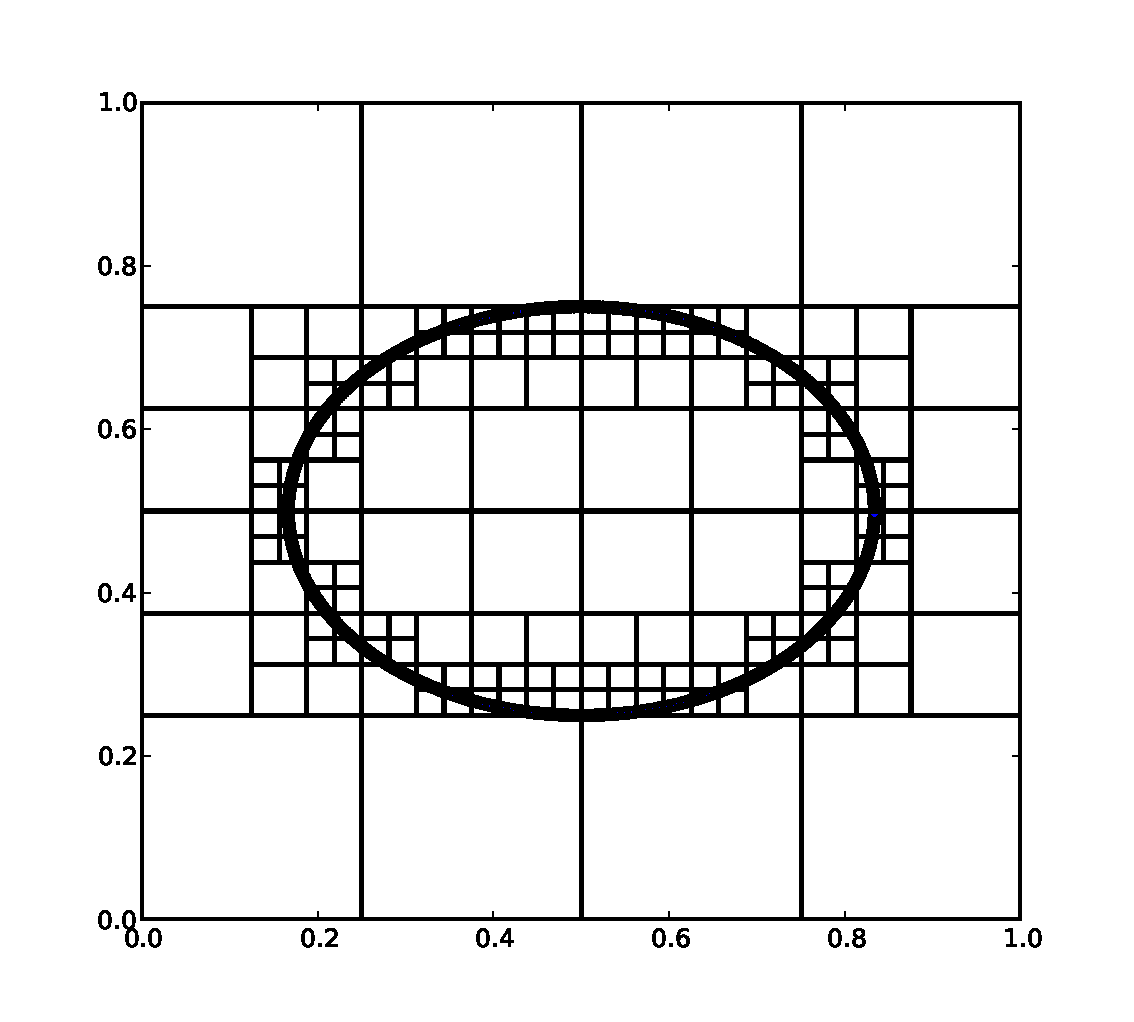
\includegraphics[bb=0in 0in 7.7in 6.3in,width=4.8in,clip]{Panels.pdf}
  \end{center}
  \caption{\small An ellipse shaped fiber $\B{X}$, with a quadtree decomposition of the space $[0,1]\times [0,1]$ containing it.}
  \label{fig:PanelDecomp}
\end{figure}

Given a panel $P$ we refer to its domain as $\Omega_{out}^P$.
A point $\B{x}$ is {\em well-separated} from a panel $P$ if  its  distance to the center of the panel is at least 3/2 the size of the panel [see~(\ref{ws})].
We refer to the domain of all points well-separated from $P$ as $\Omega_{in}^P$.
We assume that points in $\Omega_{in}^P$ are sufficiently far from $P$ that a multipole expansion could be used to calculate the effect of the {\em outgoing} influence of all the fiber points in $P$.  This assumption is equivalent to assuming that we can expand $G_h$ over $\Omega_{in}^P\times\Omega_{out}^P$, arriving at two collections of coefficient functions $\{A_k^P\}_{k=1}^p$ and $\{B_k^P\}_{k=1}^p$. 

Suppose now that we are given a fiber force $\B{F}$ and wish to evaluate its influence at points $\B{x}$ in the fluid domain. For each $\B{x}$ this influence is given by
\begin{equation}
\sum_{1\leq j\leq N_B} G_h(\B{x} - \B{X}_j) \B{F}_j.
\end{equation}
To evaluate this efficiently, we first loop over each panel $\Panel{P}$ and calculate the far field expansion of all the poles located in 
$\Panel{P}$. The $k$-th term of this expansion is given by
\begin{equation}
H_k^P \equiv \sum_{j\in B_{out}^P}
B_k^P(\B{X}_j) \tilde{F}_j.
\label{eq:Outgoing}
\end{equation}
If $\B{x}$ is well separated from $\Panel{P}$, then the incoming effect on $\B{x}$ from $\Panel{P}$ is given by
\begin{equation}
\B{E}^T \full\sum_{k=1}^{p}A_k^P(\B{X}_i)H_k^P.
\label{eq:Incoming}
\end{equation}
We can now evaluate the entire influence of $\B{F}$ on a point $\B{x}$, recursively.   We start with the panel $\Panel{P}=\Panel{Root}$. If $\B{x}$ is well separated from $\Panel{P}$ then we evaluate the influence of $\Panel{P}$ on $\B{x}$ via (\ref{eq:Incoming}). Otherwise, if $\Panel{P}$ has children we recursively apply this process to those child panels. If instead $\Panel{P}$ is childless, we directly evaluate the influence of every fiber point in $\Panel{P}$ on $\B{x}$, using (\ref{eq:SubProblem}). Summing all these influences from every branch of the recursion provides the desired total influence on $\B{x}$.

Note that (\ref{eq:Outgoing}) only needs to be calculated once per panel, and may be reused for calculating the influence at multiple points $\B{x}$. Because each fiber point $\B{X}_i$ is contained in at most $\log N$ panels, the total cost of computing $H_k^P$ for all panels $\Panel{P}$ is at most $O(N_B\log N_B)$. Calculating the influence at a given $\B{x}$ involves at most $O(\log N)$ panels, and hence the cost is at most $O(p\log N)$. The total cost of evaluating $\C{M}_n\B{F}$ is thus $O(pN_B\log N_B)$.

A detailed description of the octree creation and point evaluation is presented in~\ref{App:octree}.
\subsection{Expansions}
\label{Sec:Treecode_Expansions}
In order to make use of a treecode we must be able to find expansions (\ref{eq:Expansion}) of $G_h$ associated with particular pairs $\left(\Omega_{in},\Omega_{out}\right)$. Here, 
$G_h$ is a summation of discrete stokeslets. In free space, the continuous stokeslet has convenient analytic expansions useful for fast summation, see for instance~\cite{Stokes_FMM}. The same is not true for the discrete stokeslet corresponding to a periodic domain, and much less so for the particular summation of stokeslets that yields $G_h$. Fortunately, an analytic expansion is not indispensable in practice. What we seek are collections of tensor valued function $\{A_k\}_{k=1}^\Inf$ and $\{B_k\}_{k=1}^\Inf$ defined on $\Omega$ such that 
\begin{equation}
G_h(\B{x} - \B{y}) = \sum_{k = 1}^\infty A_k(\B{x}) B_k(\B{y}),
\end{equation}
and, moreover, such that truncating the above expansion to $p$ terms yields an adequate approximation, provided that $\B{x}$ and $\B{y}$ are well separated in some sense. That is, given two disjoint subsets $\Omega_{in}$ and $\Omega_{out}$ of our domain, we hope that for some small value of $p$ and for a specified tolerance $\epsilon$ that
\begin{equation}
\norm{
\left(G_h(\B{x} - \B{y}) - \sum_{k = 1}^p A_k(\B{x}) B_k(\B{y})\right)
\B{f}
}_2 < \epsilon \norm{\B{f}}_2,
%\text{ for $\B{x}\in\Omega_{in},\B{y}\in\Omega_{out}$},
\label{eq:Accuracy}
\end{equation}
for all $\B{f}\in\BB{R}^3$, $\B{x}\in\Omega_{in}$, and $\B{y}\in\Omega_{out}$.
%For our needs we will take $\epsilon\sim h$, the order of our discretization.

For a given $p$, finding the optimal expansion that allows for the smallest $\epsilon$ that satisfies (\ref{eq:Accuracy}) for all $\B{f},\B{x},\B{y}$ is an open question, and is likely computationally intractable.

We solve instead a least squares problem. We will search for the individual components of our tensors separately. Looking at each $ab$ components, for $a,b=x,y,z$, we seek the expansion coefficients $\{(A_k)_{ab}\}_{k=1}^p$ and $\{(B_k)_{ab}\}_{k=1}^p$ such that we minimize the $L^2$-norm of the difference between $G_h$ and our approximate expansion. That is, we seek to minimize
\begin{equation}
\norm{\left(G_h - \sum_{k = 1}^p A_k B_k\right)_{ab}}^2_2 \equiv
\iint
\left(G_h(\B{x} - \B{y}) - \sum_{k = 1}^p A_k(\B{x}) B_k(\B{y})\right)_{ab}^2
d\B{x} d\B{y},
\label{eq:L2Dif}
\end{equation}
where $A_k B_k$ is understood to be a function over $\Omega_{in}\times\Omega_{out}$, and the integrals are taken over $\B{x}\in\Omega_{in}$ and $\B{y}\in\Omega_{out}$. We approximate the integral in (\ref{eq:L2Dif}) as
\begin{equation}
\sum
\left(G_h(\B{x} - \B{y}) - \sum_{k = 1}^p A_k(\B{x}) B_k(\B{y})\right)_{ab}^2 h^6,
\label{eq:L2Dif_Sum}
\end{equation}
where the outer sum is taken over the Eulerian grid points in our subsets, $\B{x}\in\Omega_{in}\cap\C{G}_h$ and $\B{y}\in\Omega_{out}\cap\C{G}_h$.
Note that this minimization problem is decoupled with respect to the components of our tensors. We may thus consider the task of minimizing (\ref{eq:L2Dif_Sum}) as nine separate minimization problems.

It is useful to view our problem as a statement about matrices. To do this we first write $(G_h)_{ab}$ as an $N^3\times N^3$ matrix, which we refer to as $\ti{G}$ and which is given by the relation
\begin{equation}
\ti{G}_{ij} = G_h((j_0,j_1,j_2)h-(i_0,i_1,i_2)h),
\end{equation}
where $i = i_0 + i_1N + i_2N^2$ and $j = j_0 + j_1N + j_2N^2$ for any $0\leq i_l < N$, $0\leq j_l < N$, with $l=0,1,2$. We may likewise write $(A_k)_{ab}$ and $(B_k)_{ab}$ as $N^3$-vectors labeled $\ti{A}_k$ and $\ti{B}_k$.
We now stitch our collections of vectors $\{\ti{A}_k\}$ and $\{\ti{B}_k\}$ into matrices. Given $p$, we define an $N^3\times p$ matrix $U$, a $p\times N^3$ matrix $V$, and a $p\times p$ diagonal matrix $\Sigma$ via
\begin{equation}
U_{jk} = \frac{(\ti{A}_k)_j}{\norm{\ti{A}_k}_2},
\qquad
V_{kj} = \frac{(\ti{B}_k)_j}{\norm{\ti{B}_k}_2},
\qquad
\Sigma_{kk} = \norm{\ti{A}_k}_2 \norm{\ti{B}_k}_2,
\end{equation}
for $1\leq j\leq N^3$ and $1\leq k\leq p$.

The $p$ columns of $U$ are simply the normalized vector encodings of the $p$ coefficient functions $\{A_k\}_{k=1}^p$. The rows of $V$ are likewise formed from $\{B_k\}_{k=1}^p$.
Note that we may reorder our indices such that $\{\Sigma_{kk}\}_{k=1}^p$ is a decreasing sequence.

We can now express our sum (\ref{eq:L2Dif_Sum}) as $\norm{\ti{G}-U\Sigma V}_F^2h^6$, where $\norm{\cdot}_F$ is the Frobenius matrix norm. Minimizing the Frobenius norm here is a well-studied least squares problem. It is known that if we take $p=N^3$ and find the optimal expansion minimizing (\ref{eq:L2Dif_Sum}) then we recover $\ti{G}$ exactly. That is, $\ti{G} = U\Sigma V$. This is precisely the Singular Value Decomposition (SVD) of $\ti{G}$.

The key property of this decomposition for our needs is that, for a given $p<N^3$, truncating the SVD to $p$ terms provides the minimizing expansion for (\ref{eq:L2Dif_Sum}). That is, given the SVD of $\ti{G}$,
we can obtain the optimal $p$-term expansion coefficient functions $\left\{A_k\right\}_{k=1}^p, \left\{B_k\right\}_{k=1}^p$ from the first $p$ columns of $U\sqrt{\Sigma}$ and the first $p$ rows of $\sqrt{\Sigma}V$, respectively. This result is known as the Eckart-Young theorem~\cite{EckartYoung} and the resulting expansion is the so-called rank-1 decomposition.
%The phrase rank-1 decomposition is used to stress that the terms $A_i\otimes B_i$ are rank-1 functions.

Using this optimal $p$-term expansion, the $L^2$-error (\ref{eq:L2Dif_Sum}) is given by the square sum of the neglected singular values,
\begin{equation}
\left( \sum_{k=p+1}^{N^3}\Sigma_{kk}^2 \right)^{1/2}.
\end{equation}
The accuracy of our $p$-term expansion is thus directly related to the rate of decay of the singular values of $\ti{G}$. The faster the singular values decay the fewer terms we require in our expansion  to accurately capture the behavior of $\ti{G}$. Figure~\ref{fig:svalues_00} shows the sharp decay of the singular values of $\ti{G}$, where we have encoded in $\ti{G}$ the $xx$ and $xy$ components of $G_h$ respectively. It is this marked decay that allows for an efficient treecode approach.
\begin{figure}[htb]
	\begin{center}
		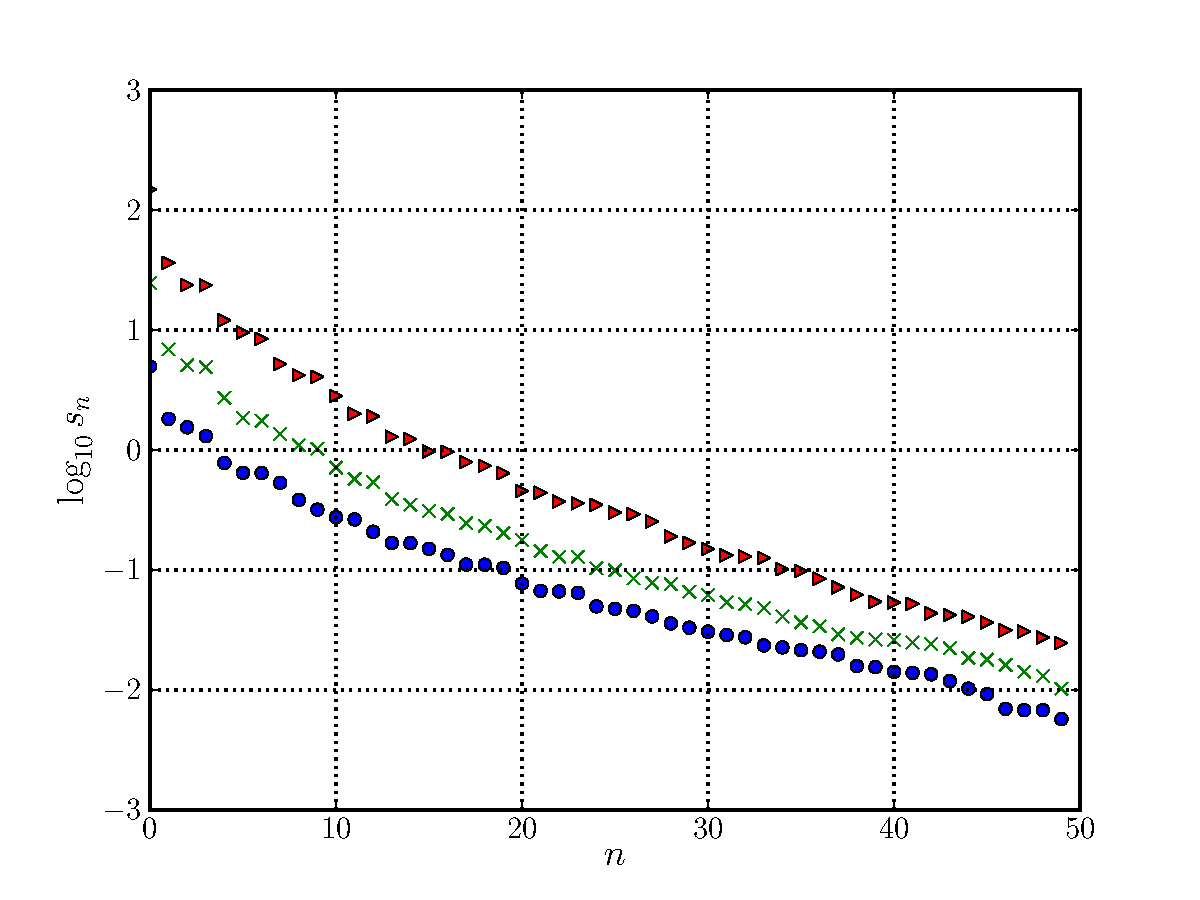
\includegraphics[bb=0in 0in 7.7in 6.3in,width=\StandardFigureWidth,clip]{svalues_00.pdf}
	\end{center}
	\begin{center}
		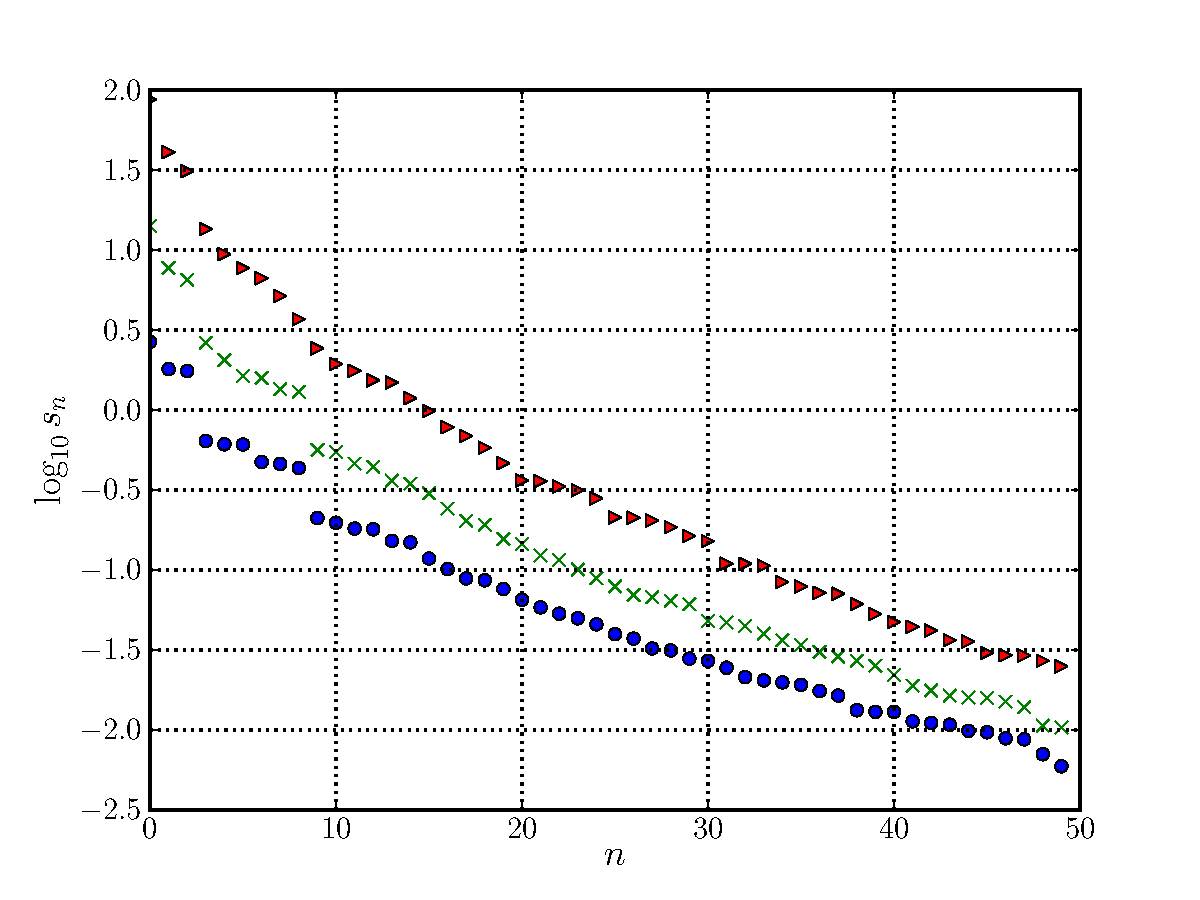
\includegraphics[bb=0in 0in 7.7in 6.3in,width=\StandardFigureWidth,clip]{svalues_01.pdf}
	\end{center}	
	\caption{Singular values of the discrete Green's function: $\left(G_h\right)_{xx}$ component (top) and $\left(G_h\right)_{xy}$ component (bottom). 'o' markers are for $N=32$, 'x' markers are for $N=64$, and '$\triangle$' makers are for $N=128$.}
	\label{fig:svalues_00}
\end{figure}

Calculating the SVD of $\ti{G}$ can be expensive. Fortunately, as with the construction of $G_h$, this is a one time cost that can be spread over multiple simulations. However, some care must still be taken as a direct approach to calculating the SVD of $\ti{G}$ would require $O(N^9)$ operations. In~\ref{Sec:Decomposition} we propose an 
efficient strategy to reduce the cost to $O(pN^3\log N)$ operations.

Finally, turning back to our original optimization problem of minimizing (\ref{eq:L2Dif}), we approximate $A_k(\B{x})$ and $B_k(\B{x})$ at arbitrary positions $\B{x}\in\Omega_{in}$ and $\B{y}\in\Omega_{out}$ by using trilinear interpolation between the surrounding Eulerian grid points. $G_h$ is smooth away from the origin, and its singular vectors are likewise smooth. Trilinear interpolation thus introduces an error of at most $O(h^2)$. For a given interaction between two fiber points we commit this error $p$ times, for a total error on the order of $O(ph^2)$. Assuming $h$ is sufficiently small, this error is smaller than the $O(h)$ error of our expansion and the $O(h)$ error of the IB Method. A numerical verification of the error rate of our expansion is presented below in Section~\ref{Sec:Teecode_Benchmarks}.
\subsection{Decomposition group}
We have seen how to arrive at a decomposition of $G_h$ over a subdomain $\Omega_{in}\times\Omega_{out}$. However, our treecode makes use of $O(N \log N)$ different subdomains. Each subdomain will require a suitable decomposition. Fortunately, we may recycle many of these decompositions for use over multiple subdomains.

Specifically, given two panels $\Panel{P}^1$ and $\Panel{P}^2$ at the same depth in our octree, we may take their expansion coefficient functions to be identical up to translation. That is, given $\B{z}\in\Omega$,
\begin{gather}
A_k^{P_1}(\B{c}^{P_1}+\B{z}) = A_k^{P_2}(\B{c}^{P_2}+\B{z}), \\
B_k^{P_1}(\B{c}^{P_1}+\B{z}) = B_k^{P_2}(\B{c}^{P_2}+\B{z}),
\end{gather}
provided the functions are defined at the points of evaluation. Here, $\B{c}^{P_i}$ denotes the center of panel $P_i$, $i=1,2$.

Due to this equivalence we only need $\log N$ decompositions: one for each level of our octree.
The total precomputational cost of calculating our lookup tables is thus $O(pN^3\log^2 N)$, and the total memory requirement is $O(pN^3\log N)$.


\subsection{Treecode benchmarks}
\label{Sec:Teecode_Benchmarks}
We present a numerical validation and performance evaluation of the treecode. To this end, we use a test problem which consists of 
an immersed, flat plate with fiber points $\mathbf{X}_i$ tethered to fixed points $\mathbf{T}$ and with a fiber force  $\C{A}_{h_B}(\B{X}) = \sigma(\B{T} - \B{X})$ (see Section~\ref{sec:TestProblems} for details on this problem setup).  We fix $N=128$, $\sigma=10^7$, $\Delta t=0.002$,  and vary $N_B$ and $p$.

 The performance of the treecode is analyzed through the performance of two different function calls: the evaluation function, which takes in a fiber force $\B{F}$ and returns the influence at every fiber point $\B{X}$; and a pre-evaluation function, which does a variety of computations used to streamline the evaluation function. The pre-evaluation function is called only once per timestep

We examine accuracy first. There are two confounding factors that degrade the accuracy of our treecode. The first is that we approximate $G_h$ as a truncated rank-1 decomposition. The second is that we introduce error into the simulation by assuming translation invariance of $G_h$. In order to analyze the first component separately we consider an immersed plate where the fiber points lie exactly on Eulerian intersection. This avoids the introduction of any error from translation.

We calculate the error according to the following procedure. We first make an $O(h)$ perturbation of the fiber $\B{X}$. This perturbation generates a force $\B{F}$ on the fiber. We then evaluate $\C{M}_n\B{F}$ using both the treecode and a direct fluid solve and take the sup norm of the difference.

The blue line in Figure~\ref{fig:Benchmark_p_MaxDif} shows the resulting decrease in error for increasing values of $p$. If we do not restrict the fiber points to Eulerian intersections then the above procedure returns a different decay line, seen as the green line in Figure~\ref{fig:Benchmark_p_MaxDif}. Note that past $p=10$ no additional reduction in error is achieved. This is the point at which the $O(h)$ error from our approximation to $G_h$ overwhelms the error introduced by using a truncated expansion. In actual simulations fiber points can not be restricted to Eulerian intersections, hence any value of $p > 10$ would be computationally wasteful.


If we fix $p=10$ and compute the error for various values of $h$ we see that it does indeed decrease at least as fast as $O(h)$, as seen in Figure~\ref{fig:Benchmark_h_MaxDif}, consistent with the error bound presented in~\ref{Sec:TranslationError}.


\begin{figure}[!b]
	\begin{center}
		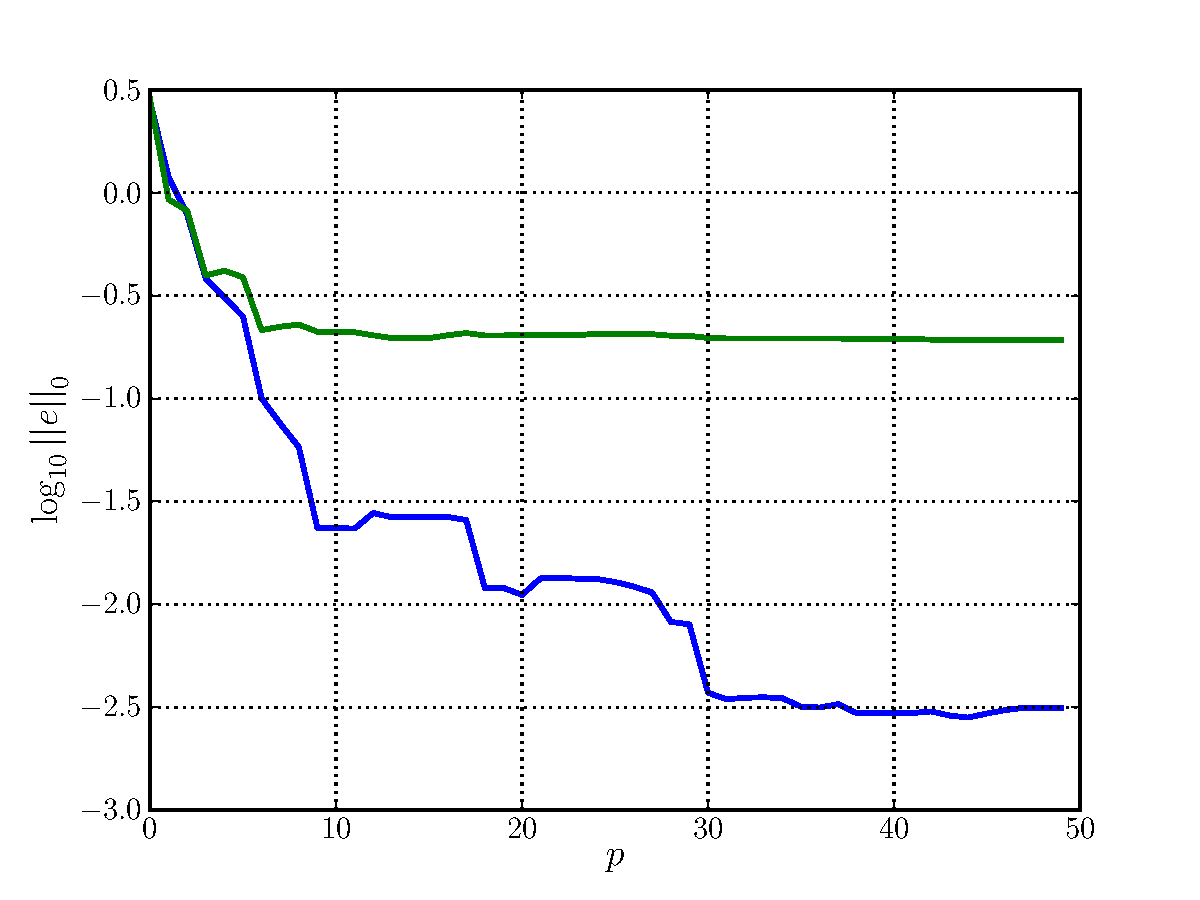
\includegraphics[bb=0in 0in 7.7in 6.3in,width=\StandardFigureWidth,clip]{Benchmark_p_MaxDif.pdf}
	\end{center}
	\caption{Log of the sup norm of the difference between $\C{M}_n\mathbf{F}$ calculated via a fluid solve and via the treecode for various values of $p$, where $p$ is the number of terms in the treecode's far field expansion. $N=128$ and $N_B=N^2/4$. The blue line is for a plate with fiber points aligned to the Eulerian grid. The green line is for a plate with no restrictions on the fiber point locations.}
	\label{fig:Benchmark_p_MaxDif}
\end{figure}

\begin{figure}[!b]
	\begin{center}
		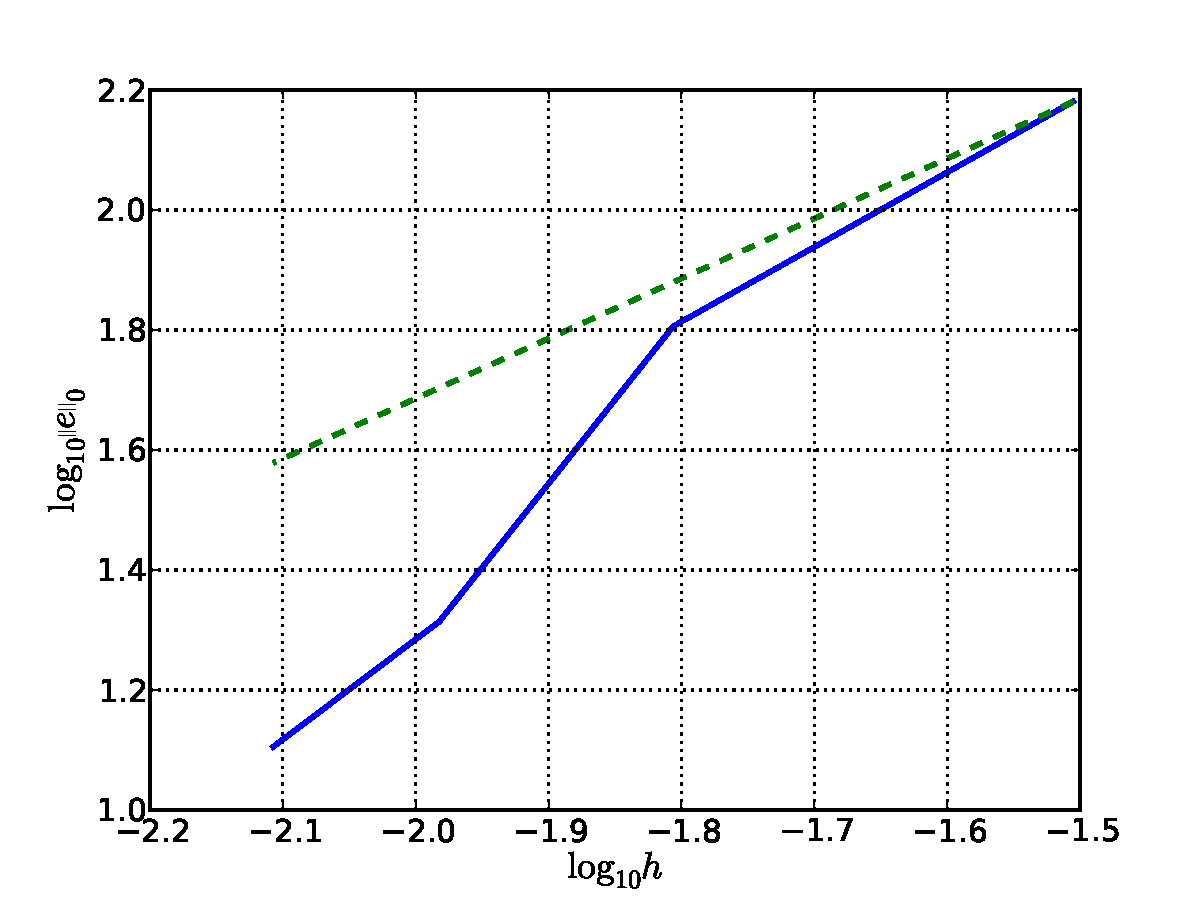
\includegraphics[bb=0in 0in 7.7in 6.3in,width=\StandardFigureWidth,clip]{Benchmark_h_MaxDif.pdf}
	\end{center}
	\caption{Log of the sup norm of the difference between $\C{M}_n\mathbf{F}$ calculated via a fluid solve and via the treecode for various values of $h$, with $p=10$. The solid blue line is the error. The dashed green line is a reference line with slope $1$.}
	\label{fig:Benchmark_h_MaxDif}
\end{figure}

We now analyze the performance of the treecode. All units of time are given as multiples of the average time to perform a fluid solve with $N=128$.
We first fix $p=10$ and vary $N_B$. The resulting CPU time for the evaluation of $\C{M}_n\B{F}$ for an arbitrary $\B{F}$ is shown in Figure~\ref{fig:Benchmark_Nb_EvalTime}. The corresponding CPU time for the pre-evaluation call is given in Figure~\ref{fig:Benchmark_Nb_PreEvalTime}. Both scale nearly linearly in $N_B$,  as expected.



\begin{figure}[!b]
	\begin{center}
		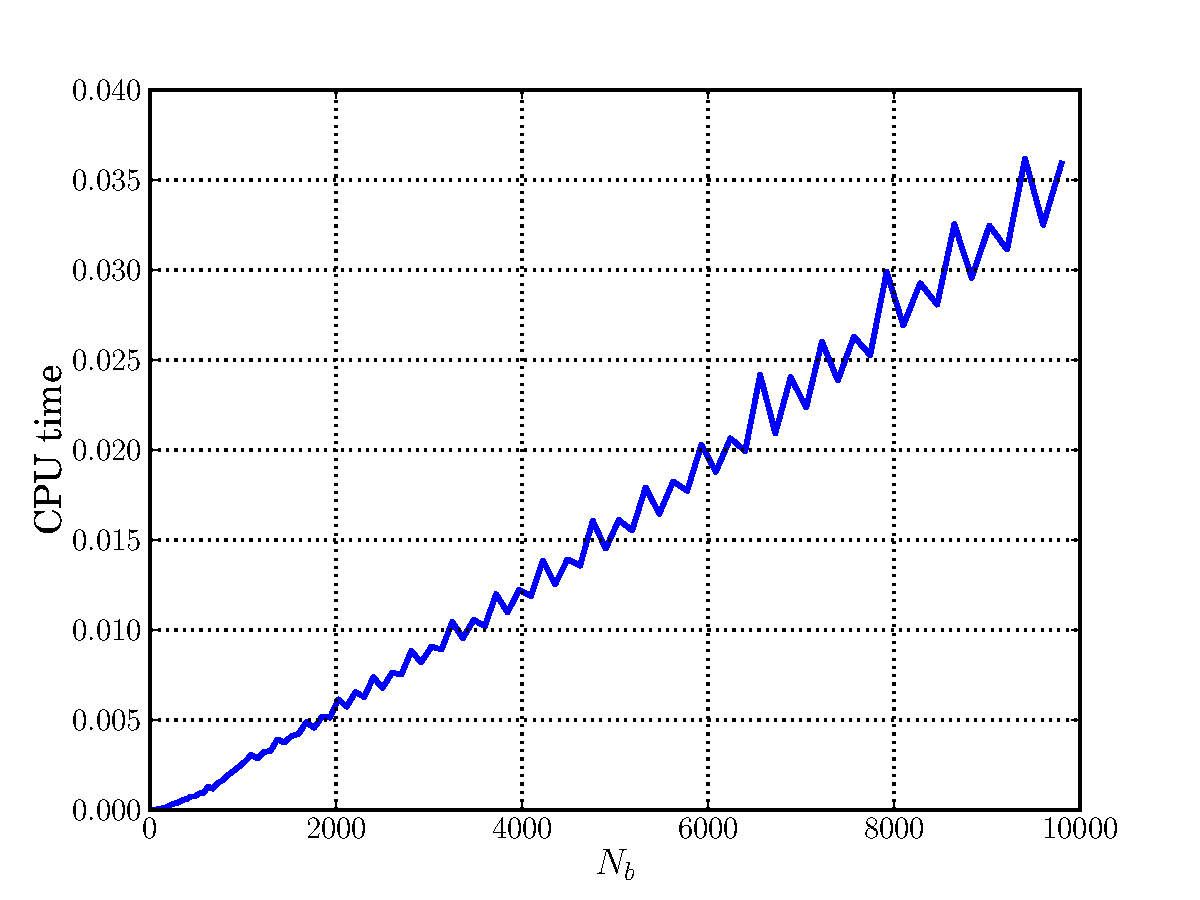
\includegraphics[bb=0in 0in 7.7in 6.3in,width=\StandardFigureWidth,clip]{Benchmark_Nb_EvalTime.pdf}
	\end{center}
	\caption{CPU time for the evaluation of $\C{M}_n\B{F}$ via the treecode for increasing values of $N_B$, where $p=10$. Time is given as multiples of the average time to perform a fluid solve, for $N=128$.}
	\label{fig:Benchmark_Nb_EvalTime}
\end{figure}

\begin{figure}[!b]
	\begin{center}
		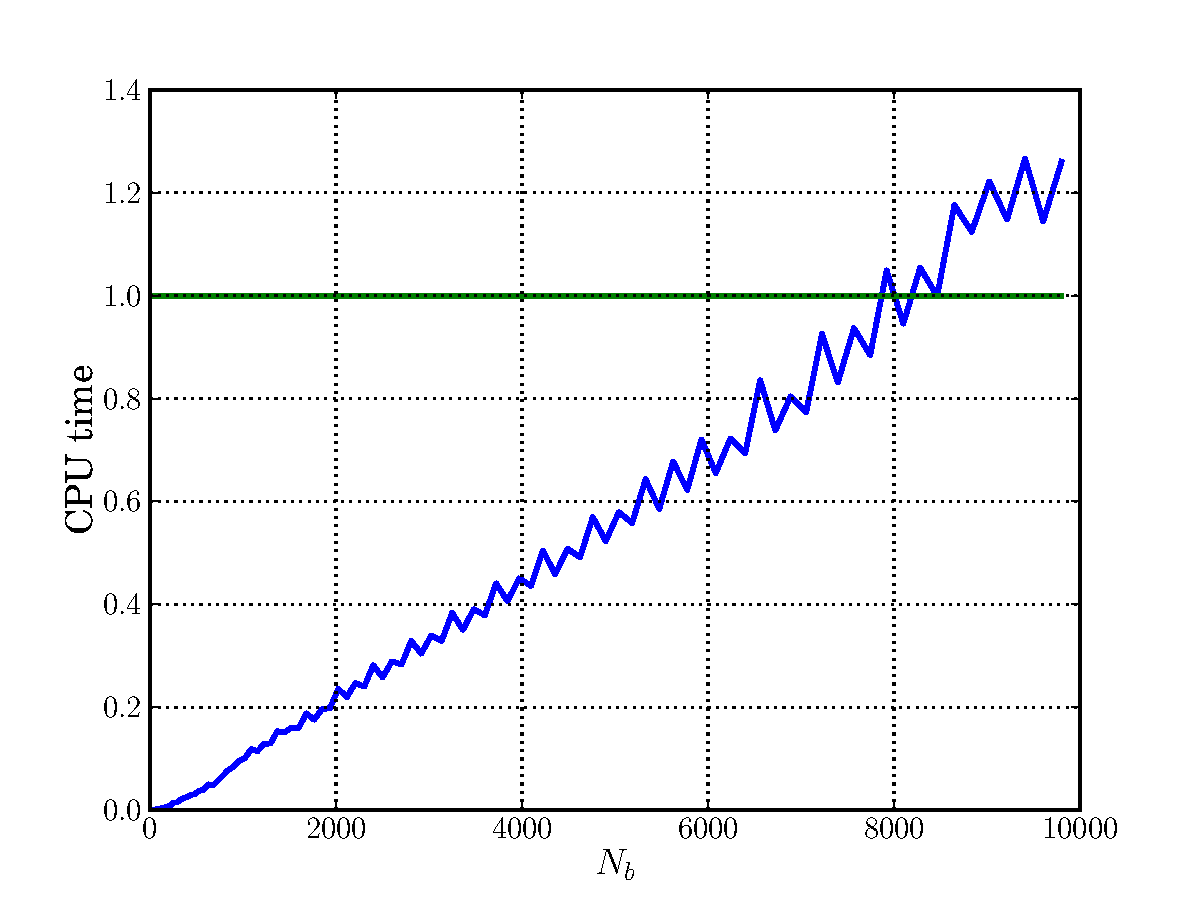
\includegraphics[bb=0in 0in 7.7in 6.3in,width=\StandardFigureWidth,clip]{Benchmark_Nb_PreEvalTime.pdf}
	\end{center}
	\caption{CPU time for the treecode pre-evaluation for increasing values of $N_B$, where $p=10$. Time is given as multiples of the average time to perform a fluid solve, for $N=128$. The green line represents the cost of one fluid solve.}
	\label{fig:Benchmark_Nb_PreEvalTime}
\end{figure}

\Comment{ % Extra tables, showing the cost of the treecode for increasing $p$
\begin{figure}[!b]
	\begin{center}
		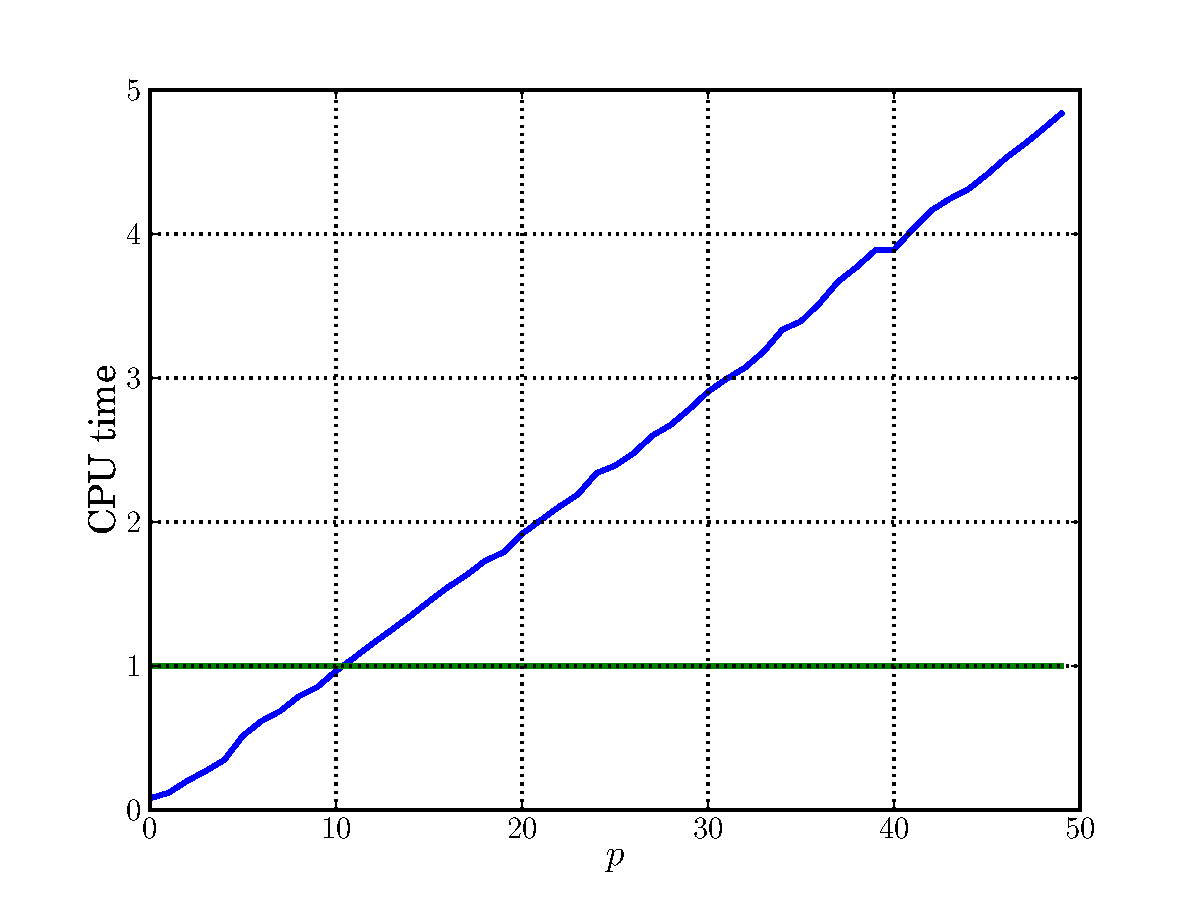
\includegraphics[bb=0in 0in 7.7in 6.3in,width=\StandardFigureWidth,clip]{Benchmark_p_PreEvalTime.pdf}
	\end{center}
	\caption{CPU time for the treecode pre-evaluation for increasing values of $p$, where $N_B=N^2/2$, $N=128$. Time is given as multiples of the average time to perform a fluid solve. The green line represents the cost of one fluid solve.}
	\label{fig:Benchmark_p_PreEvalTime}
\end{figure}

\begin{figure}[!b]
	\begin{center}
		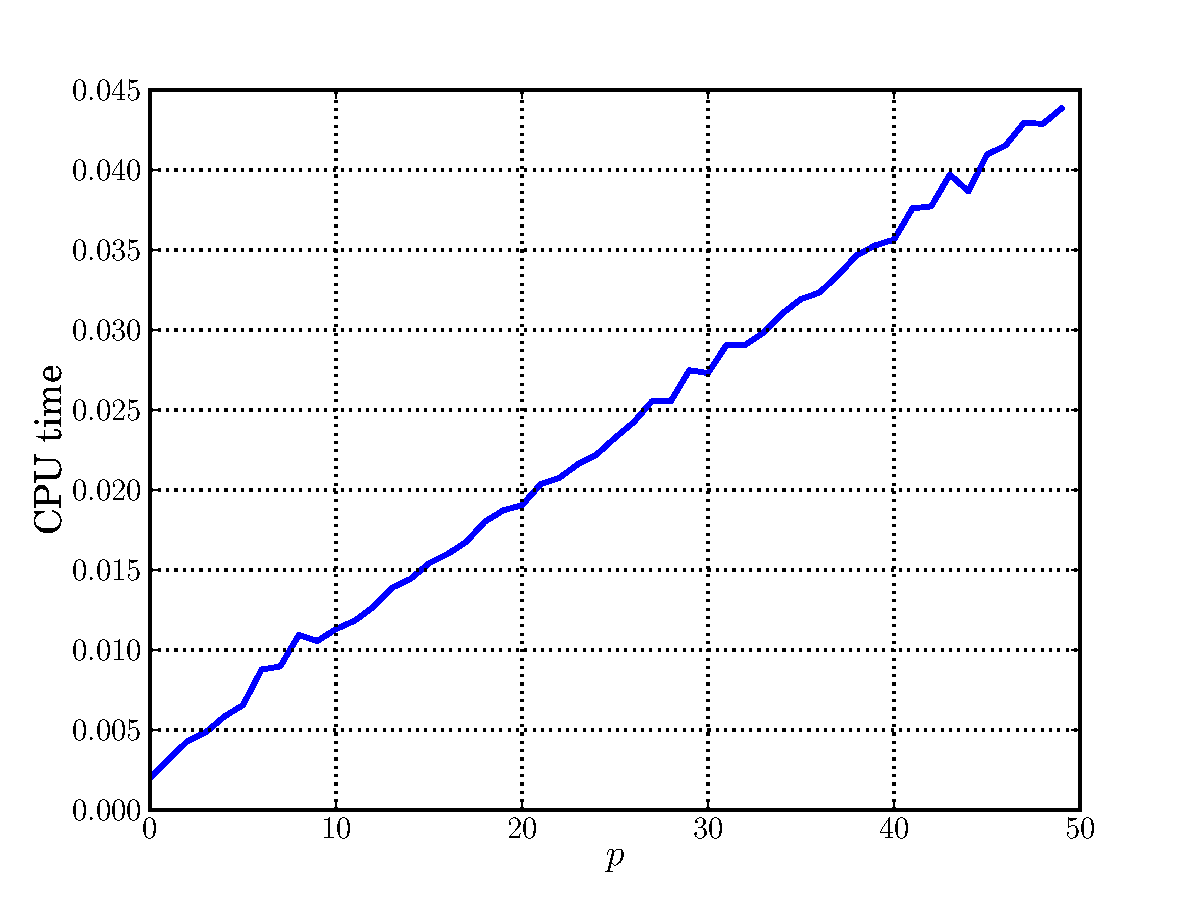
\includegraphics[bb=0in 0in 7.7in 6.3in,width=\StandardFigureWidth,clip]{Benchmark_p_EvalTime.pdf}
	\end{center}
	\caption{CPU time for the evaluation of $\C{M}_n$ via the treecode for increasing values of $p$, where $N_B=N^2/2$, $N=128$. Time is given as multiples of the average time to perform a fluid solve.}
	\label{fig:Benchmark_p_EvalTime}
\end{figure}
}


Most analytic expansions used for treecodes and FMM codes, including Taylor series expansions, are not optimal, in the sense that a different expansion would yield higher accuracy for the same number of terms. We approximate directly the $L_2$-optimal expansion. We note that the extension of treecodes and FMM codes to generic kernels, and the associated use of the SVD decomposition in particular, has been studied since the early 90s, see e.g.~\cite{SVDFMM_GimbutasEtAl} for a more detailed exposition.





\section{Numerical Results}
\label{sec:TestProblems}

\subsection{An immersed plate.}
For the first test of our proposed methodology we simulate flow past an immersed plate. The plate is a flat square of dimensions $1/2$ by $1/2$ and is discretized as an $(M+1)\times (M+1)$ grid of fiber points, where $M = \floor{N\sqrt{2}/2}$. This yields $N_B=529$, 2116, and 8281 for $N=32$, 64, and 128 respectively.

For each $j,k$ such that $0 \leq j \leq M, 0 \leq k \leq M$ we have a fiber point $\B{X}_{j,k}\in\Omega$. Each fiber point $\B{X}_{j,k}$ is tethered to a corresponding fixed point $\B{T}_{j,k}\in\Omega$ given by
\begin{equation}
\B{T}_{j,k}= (0.25,0.25,0.5) + \frac{1}{2M} (j, k, 0).
\end{equation}
The tethers induce a force $\C{A}_{h_B}(\B{X}) = \sigma(\B{T} - \B{X})$ which acts to restore the plate to equilibrium, as well as to bind the plate against the fluid flow pushing against it. The initial configuration of the plate is taken to be the equilibrium state $\B{X}^0 = \B{T}$. Note that, among non-empty Eulerian grid cells, the average number of fiber points per cell is roughly $2$. This is the minimum density needed to prevent unreasonable spurious currents across the plate.

A fluid flow is induced by adding a time dependent forcing vector $\B{f}(t)$ to the right hand side of (\ref{eq:dmoment}). We take $\B{f}(t) = 100 (0, \sin \theta(t), \cos \theta(t))$, where $\theta(t) = 4\cos(6\pi t / T) / \pi$ and $T=0.25$ is the total simulation time. The addition of $\B{f}(t)$ alters the explicit term $\B{b}^n$ in our implicit system to
\begin{equation}
\B{b}^n = \B{X}^n + \Delta t \C{S}^*_n \C{L}_h [\B{u}^n-\Delta t \B{u}^n \cdot \nabla_h \B{u}^n + \Delta t \B{f}(t^n)].
\label{eq:bn_flow}
\end{equation}
The induced flow has a Reynolds number of about 10.

$\C{A}_{h_B}$ is affine, not linear, thus we cannot directly apply CG to solve the implicit system. Suppose we denote our initial guess for $\B{X}^{n+1}$ as $\B{X}^{n+1,0}$. We define $\bar{\B{X}}^{n+1} = \B{X}^{n+1}-\B{X}^{n+1,0}$ and recast our implicit system in terms of $\bar{\B{X}}^{n+1}$. We define $\C{A}'_{h_B}(\B{X}) = -\sigma\B{X}$ and  a new explicit term
\begin{equation}
\bar{\B{b}}^n = \B{X}^n - \B{X}^{n+1,0} + \Delta t \C{S}^*_n \C{L}_h [\B{u}^n-\Delta t \B{u}^n \cdot \nabla_h \B{u}^n + \C{A}_{h_B}(\B{X}^{n+1,0}) + \Delta t \B{f}(t^n)].
\label{eq:bn_change}
\end{equation}
Our implicit system then becomes
\begin{equation}
\bar{\B{X}}^{n+1} = \C{M}_n\C{A}'_{h_B} (\bar{\B{X}}^{n+1}) + \bar{\B{b}}^n.
\label{eq:ImplicitChange}
\end{equation}
Here $\C{A}'_{h_B}$ is linear negative definite, thus $I - \C{M}_n\C{A}'_{h_B}$ is positive definite and we can solve (\ref{eq:ImplicitChange}) via CG.
\New{For CG we use a convergence tolerance of $.0001$, which is at least $10$ times smaller than the error of the method. For an initial guess we take $\B{X}^{n+1,0}=\B{X}^n$.}

We perform both explicit and implicit simulations for $N=32,64,128$ and various values of $\sigma$. 
The explicit simulation uses a standard Forward Euler/Backward Euler  (FE/BE) discretization, i.e. implicit in the viscous term but explicit in all the other terms, including the tension force. The largest stable timestep is given by the empirical formula $\Delta t = 10h\sigma^{-1/2}$.
 Table~\ref{table:ExplicitTimestep_Plate}  provides a list of the values of $\Delta t$ required for a stable simulation using the FE/BE discretization.
 Note that even for modest resolutions the timestep is prohibitively small.
\begin{table}
\caption{ $\Delta t$ in the explicit simulations of the immersed plate for various values of $N$ and $\sigma$. $\Delta t$ is approximately the largest {\em stable} timestep, given by the formula $\Delta t =10h\sigma^{-1/2}$.}
\label{table:ExplicitTimestep_Plate}
\begin{center}

\begin{tabular}{c c c c c c}
  &  $\sigma=10^7$ & $\sigma=10^8$ & $\sigma=10^9$ & $\sigma=10^{10}$ & $\sigma=10^{11}$ \\
\cline{2-6}
\multicolumn{1}{c|}{$N=32$} & \TableTopSpace
3.125\e{-5} & 9.882\e{-6} & 3.125\e{-6} & 9.882\e{-7} & 3.125\e{-7} \\
\multicolumn{1}{c|}{$N=64$}  & \TableTopSpace
1.563\e{-5} & 4.941\e{-6} & 1.563\e{-6} & 4.941\e{-7} & 1.563\e{-7} \\
\multicolumn{1}{c|}{$N=128$} & \TableTopSpace
7.813\e{-6} & 2.471\e{-6} & 7.813\e{-7} & 2.471\e{-7} & 7.813\e{-8} \\
%\cline{2-6}
\end{tabular}

\end{center}
\end{table}

In marked contrast, for the semi-implicit, lagged operators discretization a constant timesteps of $\Delta t = 0.002$ is sufficient to maintain
both stability and accuracy for all resolutions and values of $\sigma$.  Our proposed fast solution strategy yields total computation times that
are several orders of magnitude smaller than those for the popular FE/BE method. The total CPU time is shown in Table~\ref{table:SimulationTime_Plate}.
The savings are striking; computations that would take over a month to perform with the FE/BE (even with a modest $N=128$) can be done in minutes using the proposed new approach. Note also that  as $\sigma$ increases the total CPU time using the new methodology is almost invariant, whereas for the explicit FE/BE simulations the total CPU time grows markedly. 
\begin{table}
\caption{Total CPU time in hours for the explicit and implicit simulations of the immersed plate, with varying values of $\sigma$. $^*$ denotes an extrapolated value.}
\label{table:SimulationTime_Plate}
\begin{center}

\begin{tabular}{c c c c c c c}
  &  & $\sigma=10^7$ & $\sigma=10^8$ & $\sigma=10^9$ & $\sigma=10^{10}$ & $\sigma=10^{11}$ \\
\cline{3-7}
\multirow{2}{*}{$N=\hspace{1ex} 32$}
& \multicolumn{1}{c|}{Implicit} & \TableTopSpace
   0.012 & 0.011 & 0.011 & 0.013 & 0.012 \\
& \multicolumn{1}{c|}{Explicit} & \TableTopSpace
   0.214 & 0.675 & 2.146 & 6.806 & 21.296 \\
\vspace{.15 cm}
\\
  &  & $\sigma=10^7$ & $\sigma=10^8$ & $\sigma=10^9$ & $\sigma=10^{10}$ & $\sigma=10^{11}$ \\
\cline{3-7}
\multirow{2}{*}{$N=\hspace{1ex} 64$}
& \multicolumn{1}{c|}{Implicit} & \TableTopSpace
   0.109 & 0.109 & 0.106 & 0.111 & 0.108 \\
& \multicolumn{1}{c|}{Explicit} & \TableTopSpace
   4.072 & 12.906 & 40.813$^*$ & 129.063$^*$ & 408.133$^*$ \\
\vspace{.15 cm}
\\
  &  & $\sigma=10^7$ & $\sigma=10^8$ & $\sigma=10^9$ & $\sigma=10^{10}$ & $\sigma=10^{11}$ \\
\cline{3-7}
\multirow{2}{*}{$N=\hspace{1ex} 128$}
& \multicolumn{1}{c|}{Implicit} & \TableTopSpace
   0.896 & 0.889 & 0.897 & 0.892 & 0.896 \\
& \multicolumn{1}{c|}{Explicit} & \TableTopSpace
   64.779$^*$ & 204.8481$^*$ & 647.787$^*$ & 2048.481$^*$ & 6477.867$^*$ \\
\end{tabular}
   
\end{center}
\end{table}

In Table~\ref{table:ImplictTimeBreakdown} we provide a break down of the computational costs associated with a single implicit timestep for the case of the immersed plate. All units of time are given as multiples of the average time to perform a fluid solve for the given value of $N$. Of note is that the cost of performing Conjugate Gradient, typically requiring 5 to 10 iterations, is only a small contribution to the overall computational cost. The predominant costs come from the fluid solves and the treecode initialization and pre-evaluation.
\begin{table}
\caption{A break down of average CPU time for different components of the implicit timestep. Time is given as multiples of the average time to perform a fluid solve. Included in the Tree Initialization is the pre-evaluation cost.}
\label{table:ImplictTimeBreakdown}
\begin{center}

\begin{tabular}{c c c c}
%\cline{2-4}
\rule{0cm}{2.2ex}
& $N=32$ & $N=64$ & $N=128$\\
\cline{2-4}
\rule{0cm}{2.25ex}
Fluid Solves  & 2.000 & 2.000 & 2.000 \\
Tree Initialization & 1.166 & 1.125 & 1.107 \\
Conjugate Gradient            & 0.394 & 0.327 & 0.295 \\
Total         & 3.560 & 3.452 & 3.403 \\
%\cline{2-4}
\end{tabular}

\end{center}
\end{table}


Figure~\ref{fig:TimeProgression_Plate} presents a depiction of the flow using streamlines in a sequence of snapshots. A cross-section of the
 $z$-component of the velocity is also plotted below the plate. The flow has the expected periodic behavior while the structure of the plate is maintained throughout the simulation.
 \begin{figure}[htb]
	\begin{center}
		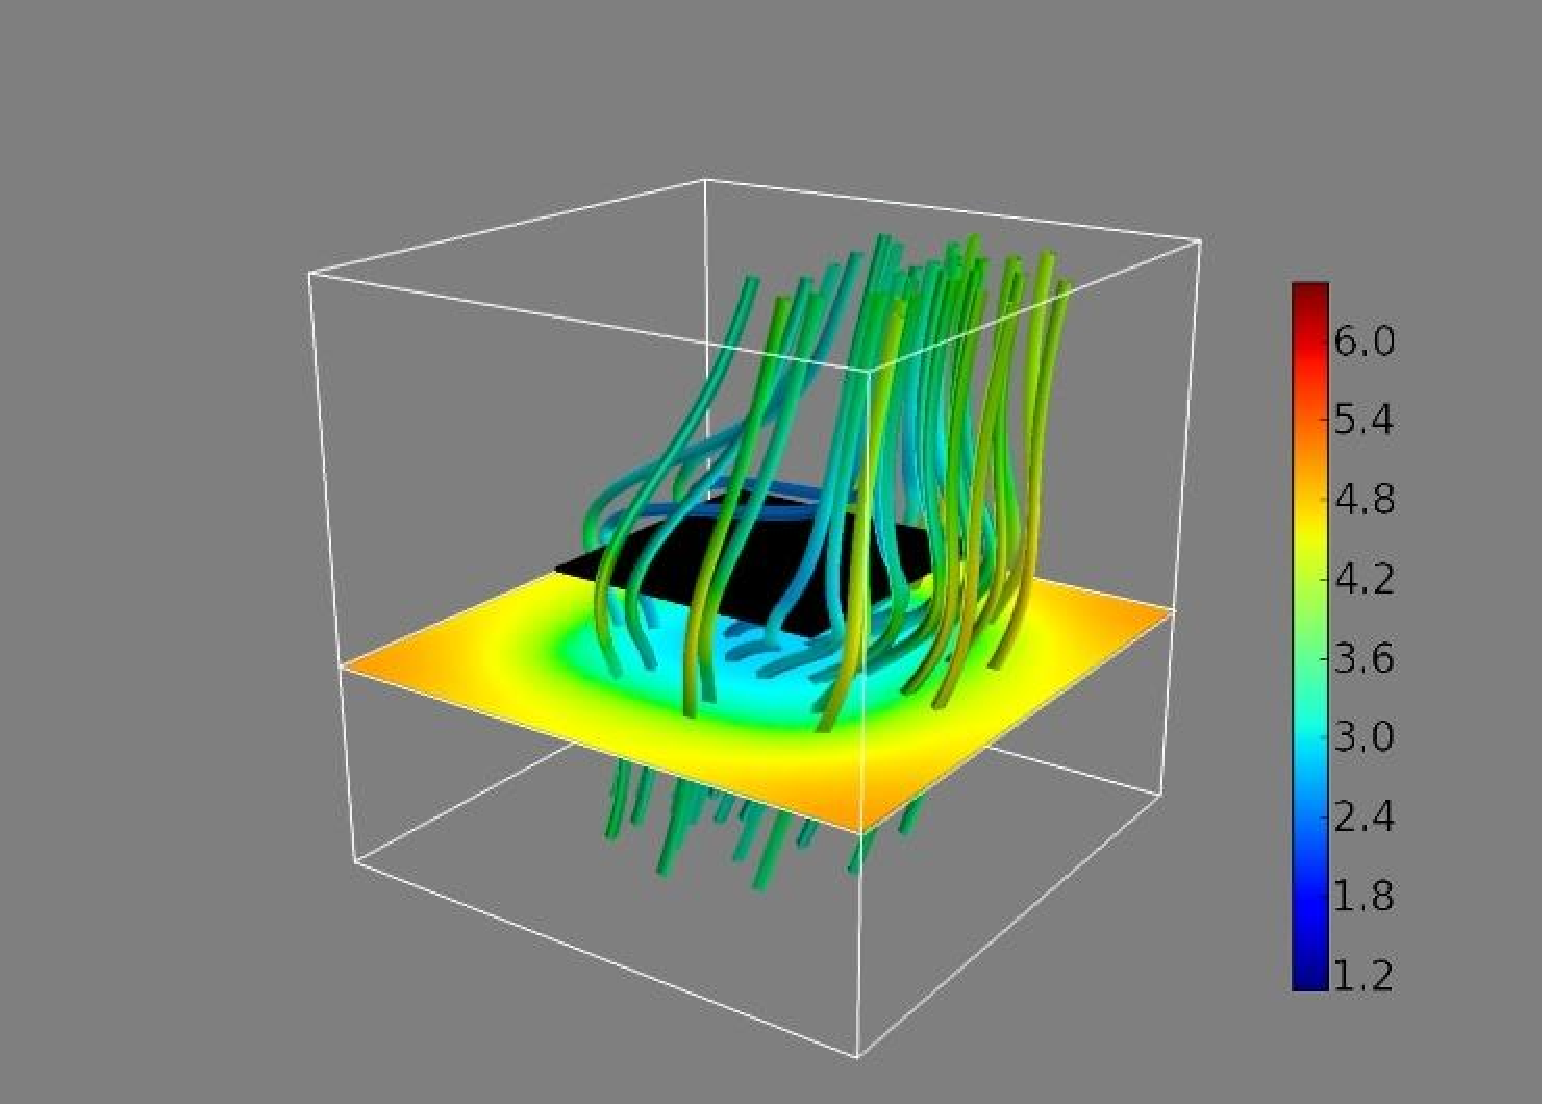
\includegraphics[bb=.0in .4in 11.5in 6.1in,width=4.355in,clip]{3dplot_50c.pdf}
		\hfill
		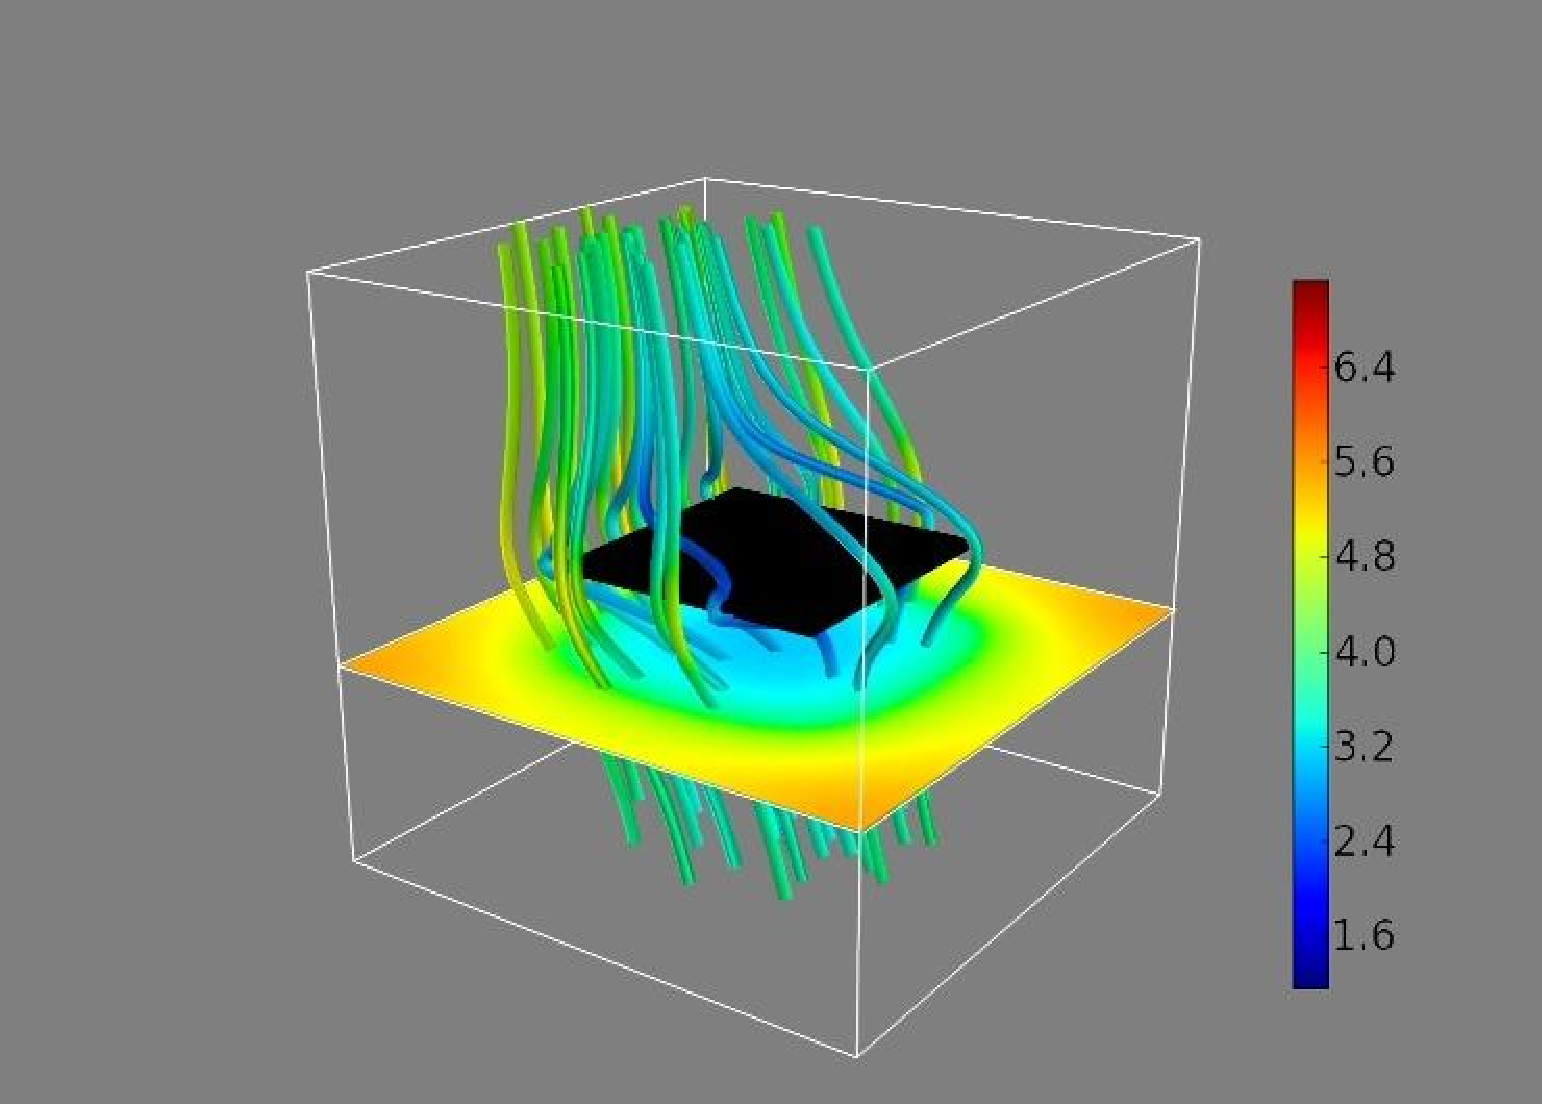
\includegraphics[bb=.0in .4in 11.5in 6.1in,width=4.35in,clip]{3dplot_72c.pdf}
		\hfill
		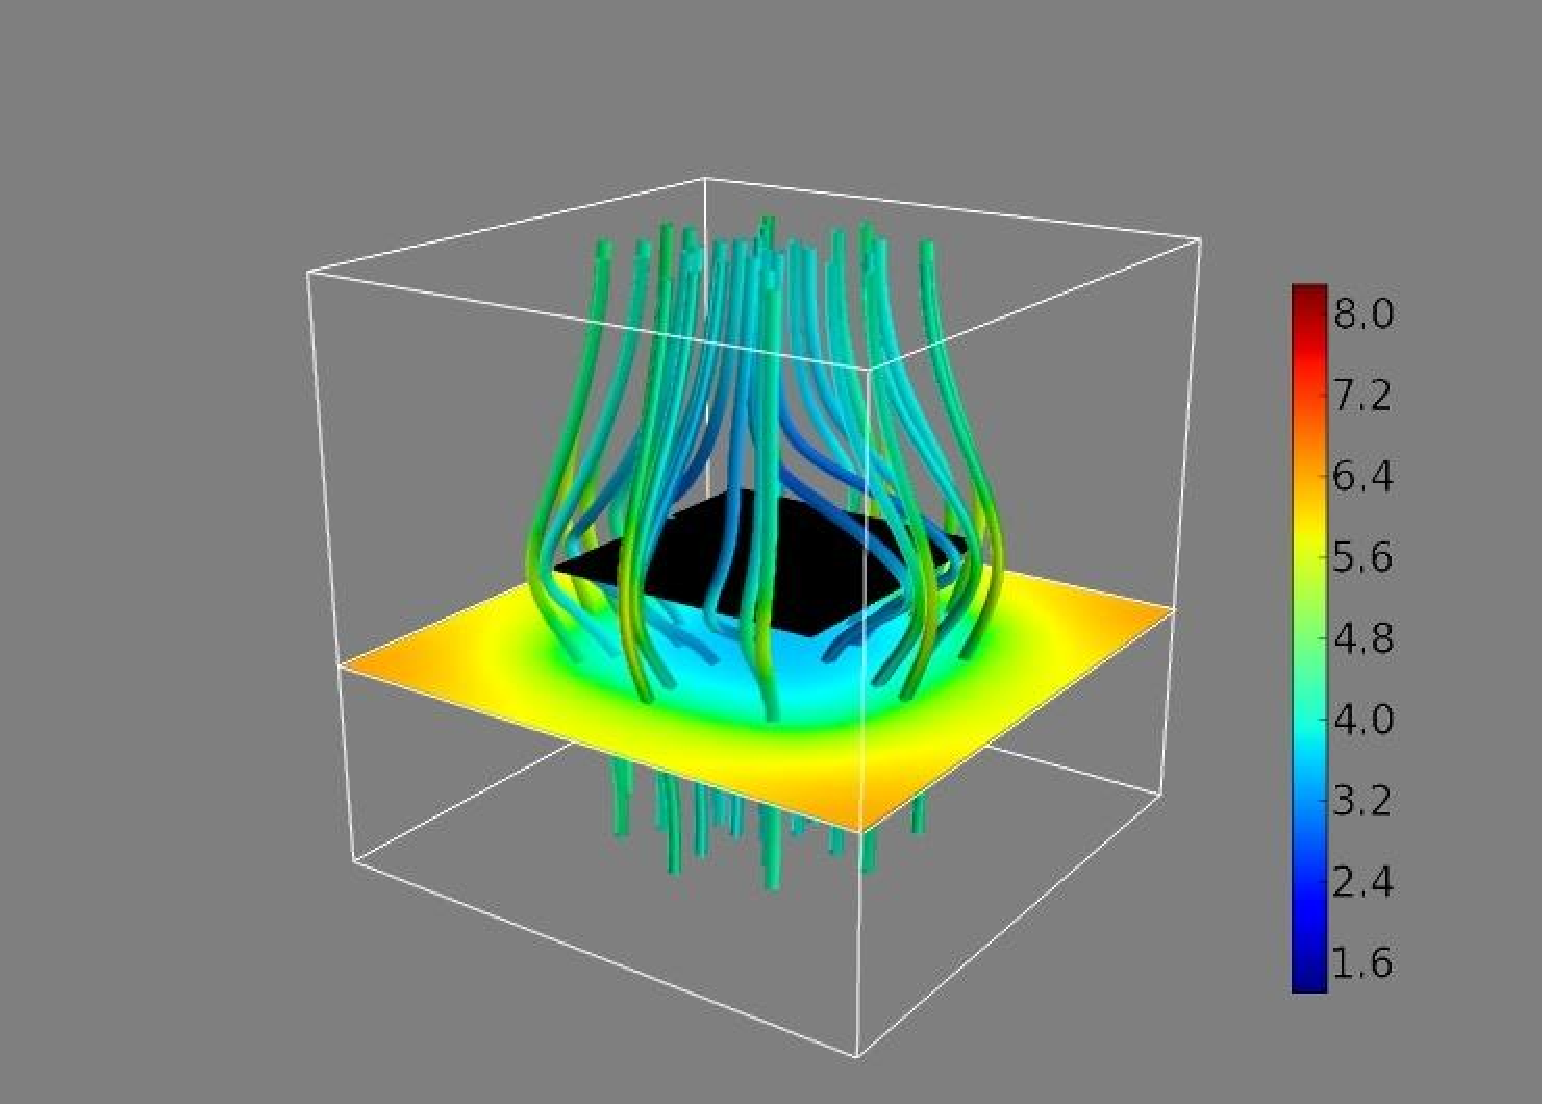
\includegraphics[bb=.0in .4in 11.5in 6.1in,width=4.355in,clip]{3dplot_104c.pdf}
	\end{center}
	\caption{\small Plot of the immersed plate with flow lines. The plate is drawn in black. Below the plate is a cross-section of the $z$-component of the velocity field with an associated color bar. $N=128$, and $N_B=8192$. Frames shown at total simulation time $T=0.020$, 0.142, and 0.208, from top to bottom.}
\label{fig:TimeProgression_Plate}
\end{figure}


\subsection{An oscillating spheroid}

In the immersed plate test described above, the geometry of the structure is trivial and the deformations are negligible. 
Of course, the true power of the IB methodology lies in its seamless handling of both rigid {\em and} dynamic, flexible interfaces and in its structure-building capability. As an example of a simulation with a dynamic, flexible  interface we consider now an immersed, oscillating spheroid
given by
\begin{equation}
\frac{(x-0.5)^2}{(0.2+0.05\sin\theta(t))^2} +
\frac{(y-0.5)^2}{(0.2+0.05\sin\theta(t))^2} +
\frac{(z-0.5-0.05\cos\theta(t))^2}{(0.2-0.1\sin\theta(t))^2} = 1,
\label{eq:SphereEqn}
\end{equation}
where $\theta(t) = 2\pi t/T$, $t$ is the current simulation time and $T=0.25$ is the total simulation time. Equation (\ref{eq:SphereEqn}) yields a spheroid centered at $(0.5,0.5,0.5+0.05\cos\theta)$ with an equatorial radius of $0.2+0.05\sin\theta$ and a polar radius of $0.2-0.1\sin\theta$.
The prescribed motion induces a flow with a Reynolds number of about 10.

The shape of the spheroid is maintained by tethers. At time $t^n$ each fiber point $\B{X}^n_j$ is tethered to its respective location on the spheroid $\B{T}^n_j$. The sphere itself is discretized by triangulating a regular octahedron, yielding $N_B=578$, 2502, and 10406 fiber points when $N=32$, 64, and 128,  respectively. When solving for $\B{X}^{n+1}$ in the semi-implicit, lagged operators discretization, we take our initial guess to be $\B{X}^{n+1,0}=\B{T}^{n+1}$.
\New{We use the same $.0001$ convergence tolerance for CG as we do in the immersed plate simulation.}

As in the previous example, we compare (explicit) FE/BE simulations with the proposed, fast, semi-implicit approach. For the FE/BE method the
stable timestep is determined by the empirical formula  $\Delta t = 0.5\cdot 10^{-1}h\sigma^{-1/2}$. Table~\ref{table:ExplicitTimestep_Sphere} provides a list of stable, explicit timesteps for this problem. 
\begin{table}
\caption{$\Delta t$ in the FE/BE explicit simulations of the immersed spheroid for various values of $N$ and $\sigma$. $\Delta t$ is approximately the largest stable timestep, given by the formula $\Delta t = 0.5\cdot 10^{-1}h\sigma^{-1/2}$.}
\label{table:ExplicitTimestep_Sphere}
\begin{center}

\begin{tabular}{c c c c c c}
  &  $\sigma=10^5$ & $\sigma=10^6$ & $\sigma=10^7$ & $\sigma=10^{8}$ & $\sigma=10^{9}$ \\
\cline{2-6}
\multicolumn{1}{c|}{$N=32$} & \TableTopSpace
4.941\e{-6} & 1.563\e{-6} & 4.941\e{-7} & 1.563\e{-7} & 4.941\e{-8} \\
\multicolumn{1}{c|}{$N=64$}  & \TableTopSpace
2.471\e{-6} & 7.813\e{-7} & 2.471\e{-7} & 7.813\e{-8} & 2.471\e{-8} \\
\multicolumn{1}{c|}{$N=128$} & \TableTopSpace
1.235\e{-6} & 3.906\e{-7} & 1.235\e{-7} & 3.906\e{-8} & 1.235\e{-8} \\
%\cline{2-6}
\end{tabular}

\end{center}
\end{table}
The required $\Delta t$  for a stable FE/BE simulation is even smaller than that in the plate example. Again, such direct, FE/BE simulations are impractical and would require a massive computational effort even for modest resolutions. 
For the implicit, lagged operators  discretization it is again sufficient to fix $\Delta t = 0.002$ to maintain both accuracy and stability for all resolutions,  $N=32$, 64, and 128. A comparison of the total CPU time for all simulations is presented in  
Table~\ref{table:SimulationTime_Sphere}. As in the plate example, the CPU time for the fast, semi-implicit simulations is almost invariant as 
 $\sigma$ increases.   The numbers are even more striking than in the preceding example; for $N=128$ and $\sigma=10^9$, the proposed approach is six orders of magnitude faster than the commonly used FE/BE approach.
\begin{table}
\caption{Total CPU time in hours for the explicit and semi-implicit simulations of the immersed spheroid, with varying values of $\sigma$. $^*$ denotes an extrapolated value.}
\label{table:SimulationTime_Sphere}
\begin{center}

\begin{tabular}{c c c c c c c}
  &  & $\sigma=10^5$ & $\sigma=10^6$ & $\sigma=10^7$ & $\sigma=10^{8}$ & $\sigma=10^{9}$ \\
\cline{3-7}
\multirow{2}{*}{$N=\hspace{1ex} 32$}
& \multicolumn{1}{c|}{Implicit} & \TableTopSpace
	0.013 & 0.015 & 0.015 & 0.016 & 0.016 \\
& \multicolumn{1}{c|}{Explicit} & \TableTopSpace
	4.405 & 13.675 & 43.467 & 135.742$^*$ & 429.701$^*$ \\
\vspace{.15 cm}
\\
  &  & $\sigma=10^5$ & $\sigma=10^6$ & $\sigma=10^7$ & $\sigma=10^{8}$ & $\sigma=10^{9}$ \\
\cline{3-7}
\multirow{2}{*}{$N=\hspace{1ex} 64$}
& \multicolumn{1}{c|}{Implicit} & \TableTopSpace
	0.127 & 0.134 & 0.140 & 0.138 & 0.137 \\
& \multicolumn{1}{c|}{Explicit} & \TableTopSpace
	83.155$^*$ & 253.626$^*$ & 822.769$^*$ & 2595.119$^*$ & 8213.271$^*$ \\
\vspace{.15 cm}
\\
  &  & $\sigma=10^5$ & $\sigma=10^6$ & $\sigma=10^7$ & $\sigma=10^{8}$ & $\sigma=10^{9}$ \\
\cline{3-7}
\multirow{2}{*}{$N=\hspace{1ex} 128$}
& \multicolumn{1}{c|}{Implicit} & \TableTopSpace
	1.057 & 1.125 & 1.141 & 1.151 & 1.167 \\
& \multicolumn{1}{c|}{Explicit} & \TableTopSpace
	1326.0$^*$ & 4170.7$^*$ & 13904.8$^*$ & 43827.9$^*$ & 134516.2$^*$ \\
\end{tabular}
   
\end{center}
\end{table}
A depiction of the flow obtained using the new fast, semi-implicit approach  is presented in Figure~\ref{fig:TimeProgression_Sphere}. 
 \begin{figure}[htb]
	\begin{center}
		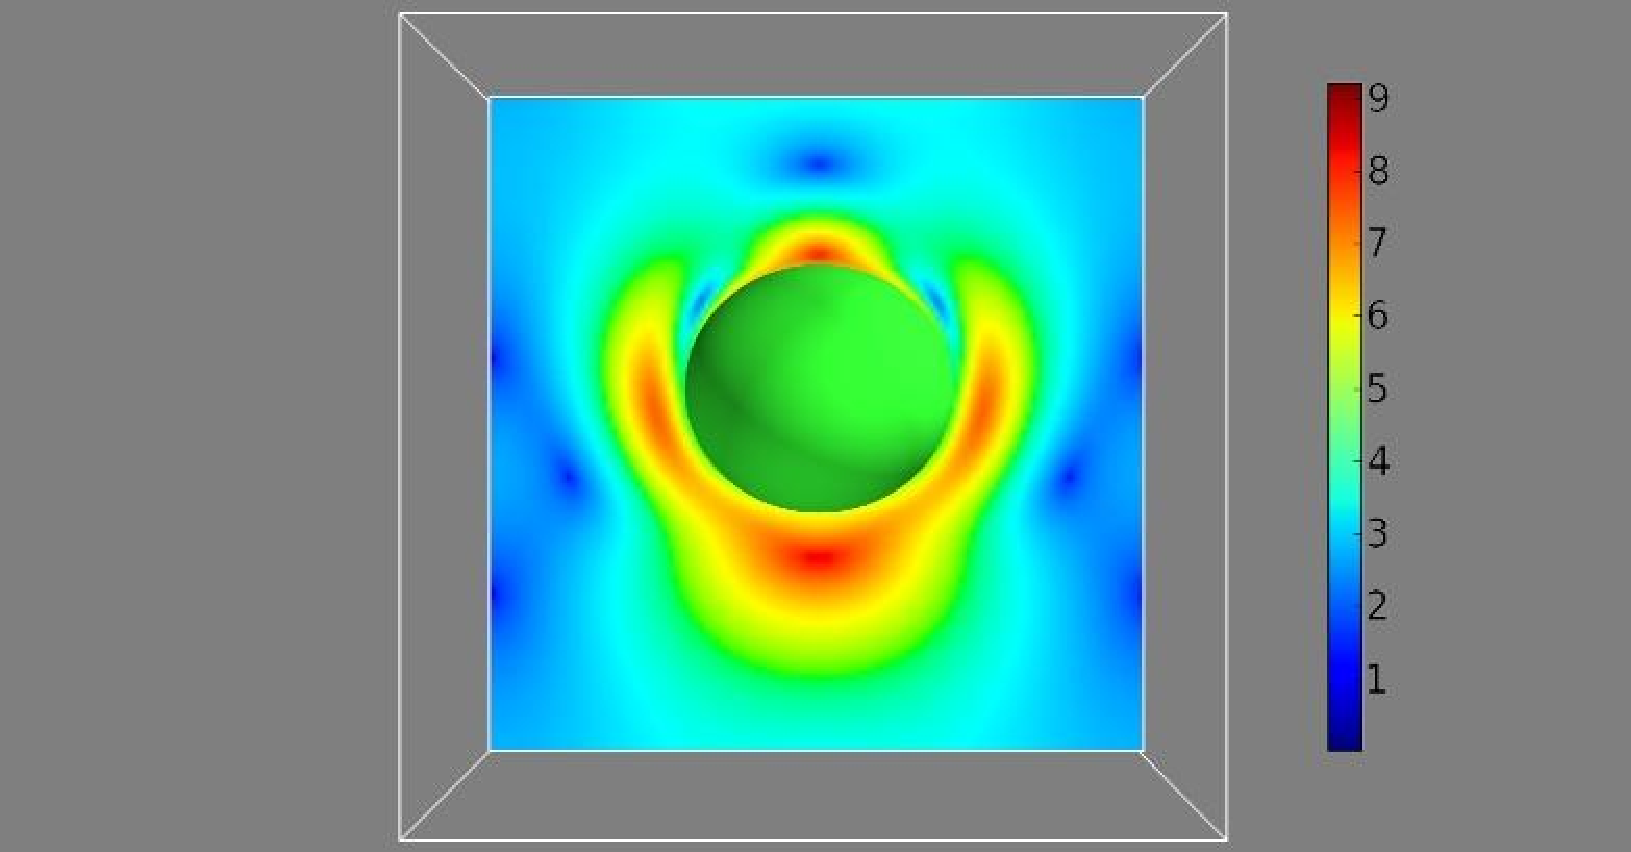
\includegraphics[bb=.0in .4in 11.5in 6.1in,width=4.4in,clip]{SpherePlot_3c.pdf}
		\hfill
		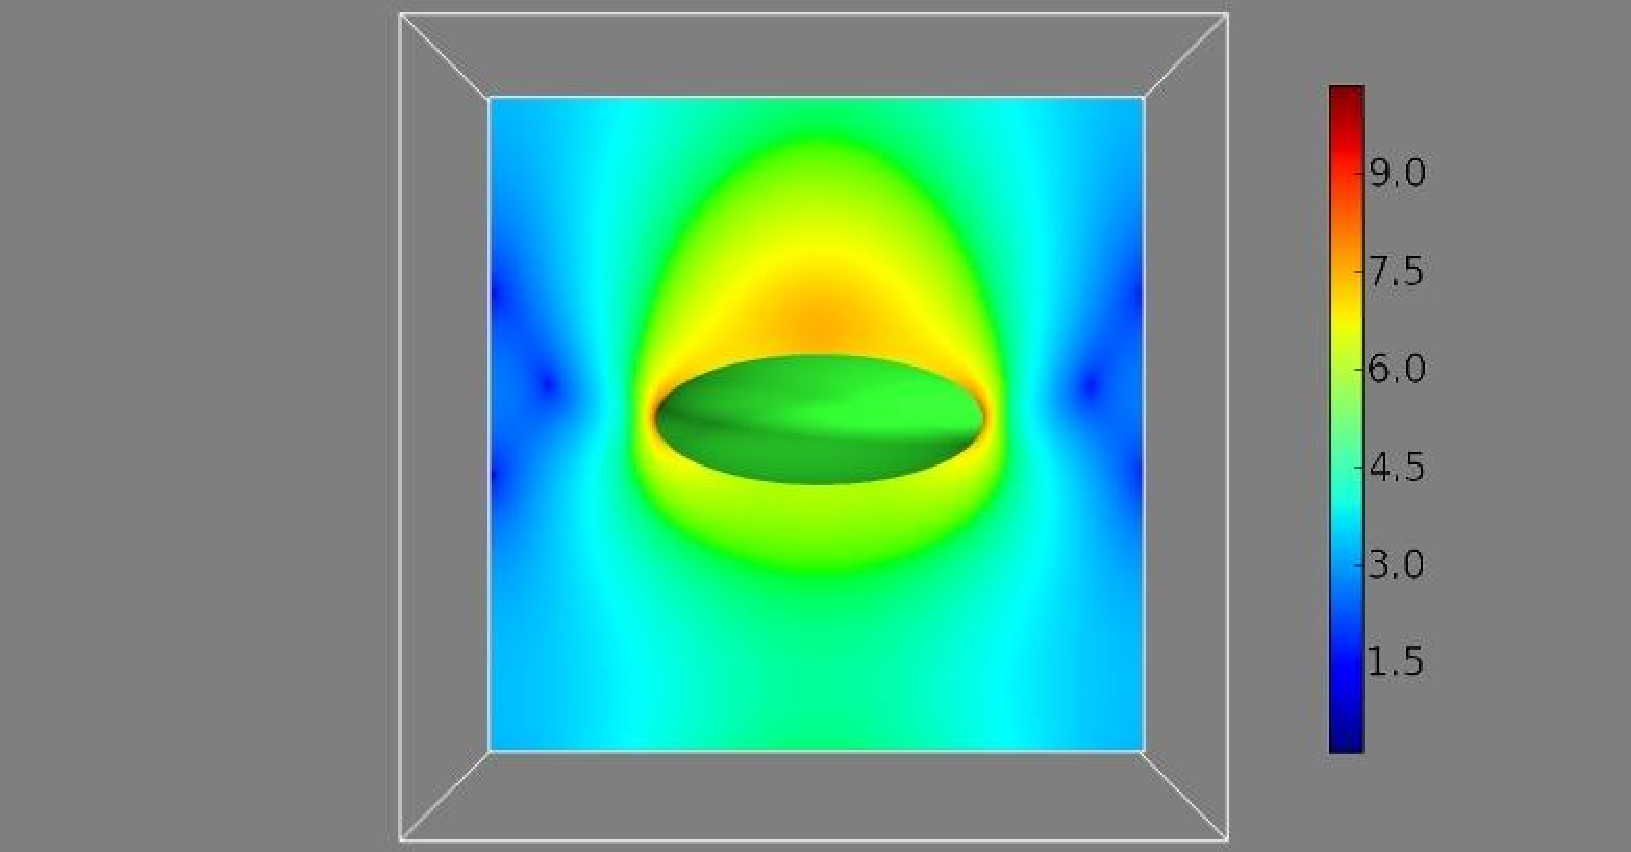
\includegraphics[bb=.0in .4in 11.5in 6.1in,width=4.4in,clip]{SpherePlot_31c.pdf}
		\hfill
		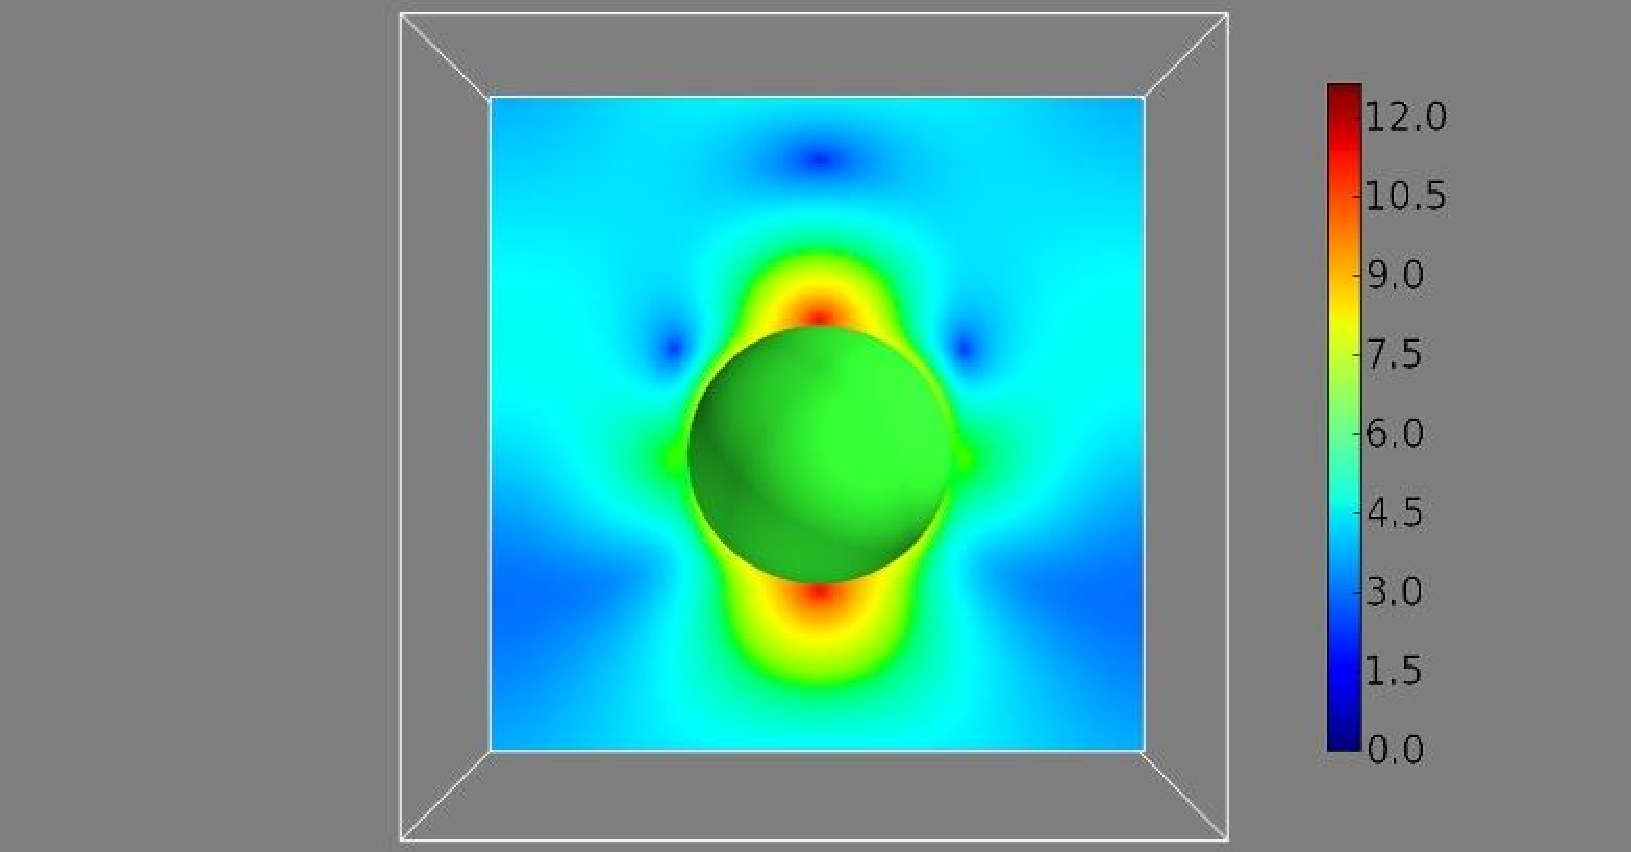
\includegraphics[bb=.0in .4in 11.5in 6.1in,width=4.4in,clip]{SpherePlot_63c.pdf}
	\end{center}
	\caption{\small Plot of the immersed spheroid, drawn in green. Cutting the spheroid is a cross-section of the velocity magnitude scalar field with an associated color bar. $N=128$, and $N_B=10406$. Frames shown at total simulation time $T=0.006$, 0.062, and 0.126, from top to bottom.}
\label{fig:TimeProgression_Sphere}
\end{figure}



\subsection{Accuracy}
There are a number of differences between our implicit methodology and the standard FE/BE explicit methodology. Each difference is a potential source of additional numerical error: the larger timestep taken, the implicit discretization itself, the assumption of translation invariance of $G_h$, the trilinear interpolation used to calculate values of the form $G_h(\B{z})$, the far field expansion of $G_h$, and approximate nature of  the Krylov subspace solvers. We have been extra careful to ensure that each of these errors is 
 no more than $O(h)$, the underlying order of the IB Method, and to verify numerically that these errors do not accumulate. 
 
To analyze error accumulation we again turn to our simulations of a plate and a sphere. For the following simulations we fix the immersed structure via tether points with spring constant $\sigma=10^6$ and induce a simple flow by adding a constant force $\B{f} = (0,0,1)$ to every point of the fluid domain. We perform the simulation first for $N=128$ using the explicit method and store the resulting fluid velocity at time $T=0.1$ as $u_{128}$. This velocity field will serve as a our standard by which we gauge the accuracy of other simulations.

We now perform the same simulation twice for $N=32$, $64$, and $96$, once using the explicit method and once using our implicit methodology. We calculate the relative error between a velocity field $\tilde{u}$ and our standard $u_{128}$ by taking the $l^2$-norm, $\norm{u_{128} - \tilde{u}}_{l^2} / \norm{u_{128}}_{l^2}$. For simplicity we downsample all velocity fields to a $32\times 32\times 32$ grid. The resulting errors can be seen in Table~\ref{table:TotalError}.

The relative errors from our implicit simulations are roughly the same as those from the explicit simulations, confirming that our fast implicit methodology is not generating any unacceptable inaccuracies.

\New{
Finally, we perform one more test to verify that approximating $G_h$ as translation invariant does not lead to a degradation of the overall accuracy. We perform a simulation using an identical setup as used for the calculation of $u_{128}$, except we shift the immersed boundary upward by a distance of $h/2$. We store the resulting fluid velocity at time $T=0.1$ as $\tilde{u}_{128}$.

If $G_h$ were exactly translation invariant then the resulting simulation would be identical to the original simulation up to a shift of the velocity field. That is, we would have $u_{128}(\B{z}) = \tilde{u}_{128}(\B{z} + (0,0,h/2))$, for any $\B{z}\in\Omega_h$. This is the case with the continuous equations.

For our discrete simulations $G_h$ is not exactly translation invariant and there is a difference between $u_{128}(\B{z})$ and $\tilde{u}_{128}(\B{z} + (0,0,h/2))$. Note that we use simple linear interpolation to calculate values of $\tilde{u}_{128}$ between grid points. 
Calculating the relative difference between $u_{128}$ and a shifted $\tilde{u}_{128}$  using the $l^2$-norm as before, we see that this difference is less than 1\%, or smaller than the error of the method. Shifts other than $(0,0,h/2)$ yield similar results.
}

\begin{table}
\caption{The relative error between various low resolution simulations and a high resolution explicit simulation.}
\label{table:TotalError}
\begin{center}

\begin{tabular}{c c c c c}
  &  & $N=32$ & $N=64$ & $N=96$ \\
\cline{3-5}
\multirow{2}{*}{Plate}
& \multicolumn{1}{c|}{Implicit} & \TableTopSpace
   0.160 & 0.0327 & 0.015 \\
& \multicolumn{1}{c|}{Explicit} & \TableTopSpace
   0.222 & 0.073 & 0.024 \\
\vspace{.15 cm}
\\
  &  & $N=32$ & $N=64$ & $N=96$ \\
\cline{3-5}
\multirow{2}{*}{Sphere}
& \multicolumn{1}{c|}{Implicit} & \TableTopSpace
	0.058 & 0.015 & 0.005 \\
& \multicolumn{1}{c|}{Explicit} & \TableTopSpace
  0.089 & 0.029 & 0.009 \\
\vspace{.15 cm}
\end{tabular}
   
\end{center}
\end{table}





\section{Conclusion}
\label{Sec:Conclusion}
In~\cite{IBM_Implicit2D}, novel expedited methods for  the semi-implicit system (\ref{eq:dmoment})-(\ref{eq:Xt}) in 2D were proposed. 
The cost of the implicit solvers therein presented were on the order of the cost of a fluid solve, allowing for efficient implicit timesteping with computational cost on the same order as that of an explicit timestep. The direct extension of that methodology to 3D proved unfeasible due to the large number of fiber points common to 3D IB applications.

In this paper, we presented an entirely new, alternative methodology suitable for the 3D case and for when there is a large number of immersed boundary point. We showed that the efficiency of the proposed  fast  semi-implicit solver,  relative to the cost of a fluid solve,  is asymptotically superior to the solvers in the 2D case. Indeed, in our test problems, we demonstrated that solving the implicit system was not the predominant cost for the semi-implicit timestep, but was rather overshadowed by the cost of the necessary fluid solves. Thus, we have  shown that the stiffness inherent in many IB applications can be eliminated via a  robust, semi-implicit discretization  for a minimal cost. More importantly, the proposed approach scales very well as $N_B$ increases, allowing the new methodology to be applied to a wide range of complex structures.
The computational savings obtained with the new methodology are enormous. IB Method computations that would typically require weeks or months using the  standard, FE/BE approach can now be performed in just minutes. 

\section*{Acknowledgments}
The authors would like to thank Profs.~Alexandre Roma and Paul J. Atzberger for insightful conversations about this work.  
Partial support for this work was provided by the National Science Foundation under Grant number DMS 1016310. 


\appendix
\section{The octree}
\label{App:octree}
Note that for this appendix we adopt a more programmatic syntax, replacing $\Omega_{in}^P$ with $\Panel{P}.\Omega_{in}$, $\B{c}^P$ with $\Panel{P}.\B{c}$, and so on. This is to facillitate the exposition of pseudocode.

We start by defining the notion of a \textit{panel}. A panel is simply a cubic subset of $\Omega$, together with an optional collection of 8 child panels that divide the parent into equal octants. Let $\Panel{P}$ be a panel. To $\Panel{P}$ we associate three vectors, $\Panel{P}.\B{c}, \Panel{P}.\B{a}, \Panel{P}.\B{b} \in\Omega$. $\Panel{P}.\B{a}$ and $\Panel{P}.\B{b}$ serve to define the domain of $\Panel{P}$, given by
\begin{equation}
\Panel{P}.\Omega_{out} = 
[\Panel{P}.\B{a}_0, \Panel{P}.\B{b}_0]\times
[\Panel{P}.\B{a}_1, \Panel{P}.\B{b}_1]\times
[\Panel{P}.\B{a}_2, \Panel{P}.\B{b}_2] \subseteq \Omega.
\end{equation}
The center of $\Panel{P}$ is denoted $\Panel{P}.\B{c} = (\Panel{P}.\B{a} + \Panel{P}.\B{b}) / 2$. This will be the center of expansion for poles inside $\Panel{P}$. We also associate to $\Panel{P}$ a collection of fiber points $\Panel{P}.\B{Y}$ consisting of those points of the fiber configuration $\B{X}$ lying within the domain $\Panel{P}.\Omega_{out}$. The children of $\Panel{P}$, if it has any, are denoted by $\Panel{P}.Child[i]$, for $0\leq i<8$. The children divide $\Panel{P}.\Omega_{out}$ equally, by splitting it into $8$ pieces via the 3 planes $x=\Panel{P}.\B{c}_0$, $y=\Panel{P}.\B{c}_1$, and $z=\Panel{P}.\B{c}_2$.

Given a domain $\Omega = [0,1]^3$, we define an initial panel called $\Panel{Root}$, specified by the bounds $\Panel{Root}.\B{a} = (0,0,0)$ and $\Panel{Root}.\B{b} = (1,1,1)$. We now recursively define child panels, creating the $8$ children of $\Panel{Root}$, then the $8$ children of each of those children, and so on. For a panel $\Panel{P}$ with few fiber points in its domain, say $|\Panel{P}.\B{Y}| < MinPoints$, we truncate the recursive process, leaving $\Panel{P}$ childless. For a pseudocode version of this process, see Function~\ref{func:Create}~CreatePanel. For our simulations we take $MinPoints = 10$. A rigorous accounting of the treecode costs can lead to an optimal value of $MinPoints$, but we did not pursue such an analysis here.

The totality of $\Panel{Root}$ and all of its branches is collectively known as the octree. 
We now introduce the concept of \textit{well separatedness}. Given a point $\B{x}$ and a panel $\Panel{P}$ we say that $\B{x}$ is well separated from $\Panel{P}$ provided that 
\begin{equation}
|\B{x}_i - \Panel{P}.\B{c}_i| \geq 3(\Panel{P}.\B{c}_i - \Panel{P}.\B{a}_i), \qquad\text{for $i=0,1,2$}, \label{ws}
\end{equation}
that is, provided that $\B{x}$ is sufficiently far from the center of $\Panel{P}$. We now consider the pair of subsets $(\Panel{P}.\Omega_{in}, \Panel{P}.\Omega_{out})$, where $\Panel{P}.\Omega_{in}$ is the collection of points in $\Omega$ that are well separated from $\Panel{P}$. We assume that we can expand $G_h$ over $\Panel{P}.\Omega_{in}\times\Panel{P}.\Omega_{out}$, arriving at two collections of coefficient functions $\{\Panel{P}.A_k\}_{k=1}^p$ and $\{\Panel{P}.B_k\}_{k=1}^p$. In addition,  we define
\begin{equation}
\Panel{P}.B_{out} = \{i\in B | \B{X}_i\in\Panel{P}.\B{Y}\},
\end{equation}
as the collection of indices associated with fiber points in $\Panel{P}.\B{Y}$. 

Suppose now that we are given a fiber force $\B{F}$ and wish to evaluate its influence at points $\B{x}$ in the fluid domain. For each $\B{x}$ this influence is given by
\begin{equation}
\sum_{1\leq j\leq N_B} G_h(\B{x} - \B{X}_j) \B{F}_j.
\end{equation}
To evaluate this efficiently, we first loop over each panel $\Panel{P}$ and calculate the far field expansion of all the poles located in $\Panel{P}.\Omega_{out}$. The $k$-th term of this expansion is given by
\begin{equation}
\Panel{P}.H_k \equiv \sum_{j\in \Panel{P}.B_{out}}
\Panel{P}.B_k(\B{X}_j) \tilde{F}_j.
\label{eq:OutgoingA}
\end{equation}
If $\B{x}$ is well separated from $\Panel{P}$, then the incoming effect on $\B{x}$ from $\Panel{P}$ is given by
\begin{equation}
\B{E}^T \full\sum_{k=1}^{p}\Panel{P}.A_k(\B{X}_i)\Panel{P}.H_k.
\label{eq:IncomingA}
\end{equation}
We can now evaluate the entire influence of $\B{F}$ on a point $\B{x}$. The process is best described in recursive form. A pseudocode is presented in Function~\ref{func:Eval}~Evaluate. 

Because our treecode must be invoked multiple times per timestep, it is critical to streamline its evaluation. There are two key points to keep in mind. First, calculations of the expansion coefficients can be recycled. In Section~\ref{Sec:Treecode_Expansions} we will detail the form of the coefficient functions $A_k$ and $B_k$. Each evaluation requires an expensive trilinear interpolation. Avoiding duplications of these calculations provides substantial speedup. Second, using the treecode to evaluate the influence at a particular point $\B{x}$ requires traversing the octree. This traversal can be stored as a template so that additional evaluations at $\B{x}$ do not require a recursive call.

There are thus two different function calls: the actual evaluation function, which takes in a fiber force $\B{F}$ and returns the influence over the entire structure $\B{X}$; and a pre-evaluation function, which does a variety of computations used to streamline the evaluation function. The cost of the pre-evaluation function is much higher than that of the evaluation function itself. However, the pre-evaluation function is called only once per timestep.

We mention one further implementation detail regarding the treatment of the domain $\Panel{P}.\Omega_{in}$ for a given panel $\Panel{P}$. Rather than treating this is as a single domain,  we break it into eight equally sized pieces, corresponding to the eight octants around the panel's center $\Panel{P}.\B{c}$. For each piece we must then have separate collections of coefficient functions $\{\Panel{P}.A_k\}_{k=1}^{p}$, $\{\Panel{P}.B_k\}_{k=1}^{p}$, as well as a separate expansion $\{\Panel{P}.H_k\}_{k=1}^{p}$.

This additional detail may seem costly at first, but in fact it increases the speed of the treecode substantially. By restricting our attention to a smaller domain it is possible to find expansions which converge much more rapidly.

\begin{algorithm}
\caption{CreatePanel$(\B{a}, \B{b})$}
\label{func:Create}
\begin{algorithmic}
\STATE $\Panel{P} \gets \B{new} \, Panel$
\STATE $\Panel{P}.\B{a} = \B{a}$
\STATE $\Panel{P}.\B{b} = \B{b}$
\STATE $\Panel{P}.\B{c} = (\B{a} + \B{b}) / 2$
\IF {$\Panel{P}.Parent$ exists}
	\STATE $\Panel{P}.\B{Y} = \Panel{P}.Parent.\B{Y} \cap \Panel{P}.\Omega_{out}$
\ELSE
	\STATE $\Panel{P}.\B{Y} = \B{X}^n \cap \Panel{P}.\Omega_{out}$
\ENDIF
\IF {$|\Panel{P}.\B{Y}| > MinPoints$}
	\STATE $ \Panel{P}.Child[0] = \text{CreatePanel}(
	\Panel{P}.\B{a},
	\Panel{P}.\B{c})$
	\STATE $ \Panel{P}.Child[1] = \text{CreatePanel}(
	[\Panel{P}.\B{c}_0, \Panel{P}.\B{a}_1, \Panel{P}.\B{a}_2] ,
	[\Panel{P}.\B{b}_0, \Panel{P}.\B{c}_1, \Panel{P}.\B{c}_2] )$
	\STATE $ \Panel{P}.Child[2] = \text{CreatePanel}(
	[\Panel{P}.\B{a}_0, \Panel{P}.\B{c}_1, \Panel{P}.\B{a}_2] ,
	[\Panel{P}.\B{c}_0, \Panel{P}.\B{b}_1, \Panel{P}.\B{c}_2] )$
	\STATE $ \Panel{P}.Child[3] = \text{CreatePanel}(
	[\Panel{P}.\B{c}_0, \Panel{P}.\B{c}_1, \Panel{P}.\B{a}_2] ,
	[\Panel{P}.\B{b}_0, \Panel{P}.\B{b}_1, \Panel{P}.\B{c}_2] )$
	\STATE $ \Panel{P}.Child[4] = \text{CreatePanel}(
	[\Panel{P}.\B{a}_0, \Panel{P}.\B{a}_1, \Panel{P}.\B{c}_2] ,
	[\Panel{P}.\B{c}_0, \Panel{P}.\B{c}_1, \Panel{P}.\B{b}_2] )$
	\STATE $ \Panel{P}.Child[5] = \text{CreatePanel}(
	[\Panel{P}.\B{c}_0, \Panel{P}.\B{a}_1, \Panel{P}.\B{c}_2] ,
	[\Panel{P}.\B{b}_0, \Panel{P}.\B{c}_1, \Panel{P}.\B{b}_2] )$
	\STATE $ \Panel{P}.Child[6] = \text{CreatePanel}(
	[\Panel{P}.\B{a}_0, \Panel{P}.\B{c}_1, \Panel{P}.\B{c}_2] ,
	[\Panel{P}.\B{c}_0, \Panel{P}.\B{b}_1, \Panel{P}.\B{b}_2] )$
	\STATE $ \Panel{P}.Child[7] = \text{CreatePanel}(
	\Panel{P}.\B{c},
	\Panel{P}.\B{b})$
\ENDIF
\RETURN $\Panel{P}$
\end{algorithmic}
\end{algorithm}

\begin{algorithm}
\caption{Evaluate$(\B{x}, \Panel{P})$}
\label{func:Eval}
\begin{algorithmic}
\IF [$\B{x}$ is well separated from $\Panel{P}$] {$\B{x} \in \Panel{P}.\Omega_{in}$}
	\RETURN $\B{E}^T \full\sum_{k=1}^{p}\Panel{P}.A_k(\B{X}_i)\Panel{P}.H_k$
\ELSE
	\IF {$\Panel{P}$ has children}
		\STATE $S = 0$ \COMMENT{the $3\times 3$ zero tensor}
		\FOR {$i = 0$ to $7$}
			\STATE $S = S + \text{Evaluate}(\B{x}, \Panel{P}.Child[i])$
		\ENDFOR
		\RETURN S
	\ELSE[do a direct summation]
		\RETURN $\full\sum_{j\in \Panel{P}.B_{out}} G_h(\B{x}, \B{X}_j) \B{F}_j$
	\ENDIF
\ENDIF
\end{algorithmic}
\end{algorithm}

\section{Computing the far field expansions}
\label{Sec:Decomposition}

\subsection{Precomputing the $G_h$ lookup table}
In Section~\ref{Sec:Treecode}, we derived the componentwise definition of $\C{M}_n$ as 
\begin{equation}
(\C{M}_n\B{F})_i \approx \sum_{0\leq j\leq N_B} G_h(\B{X}_j - \B{X}_i) \B{F}_j, \qquad\text{for $0\leq i\leq N_B$}.
\end{equation}
This requires evaluation of the function $G_h$, defined in (\ref{eq:GreensDef}). To perform this evaluation efficiently we first precompute the values of $G_h$ on our Eulerian grid $\C{G}_h$. We refer to the resulting tensor field over $\C{G}_h$ as a lookup table. The steps for creating the lookup table are as follows.
\begin{enumerate}
\item
First, we spread a unit force $\B{e}_i$ at the origin, obtaining a force field defined as $\B{e}_i \delta(\B{x})$ at any $\B{x}\in\C{G}_h$.
\item
We calculate the influence of this force field on the fluid velocity by applying the operator $\C{L}_h$, obtaining the vector field $\B{u}_{\B{0}}^i \equiv \C{L}_h( \B{e}_i \delta_h )$.
\item
We spread the velocity $\B{u}_{\B{0}}^i$ at every point $\B{x}\in \C{G}_h$, defining
\begin{equation}
(G_h(\B{x}))_i \equiv \alpha h_B \, \sum_{\B{z} \in \C{G}_\Omega} \B{u}_{\B{0}}^i(\B{z}) \delta_h\left(\B{z}-\B{x}\right)h^3.
\end{equation}
\item
Repeating the above for $i=0,1,2$, we arrive at our $3\times 3$ tensor lookup table $G_h$ over $\C{G}_h$.
\end{enumerate}
We can now rapidly evaluate terms of the form $G_h(\B{X}_j - \B{X}_i)$ by looking up the value of $\B{X}_j - \B{X}_i$ on our lookup table. For vectors that do not lie exactly on an Eulerian intersection we make use of trilinear interpolation.

\subsection{Calculating a truncated SVD of restrictions of $G_h$}
The far field expansions of $G_h$ that we employ are known as rank-1 decompositions, and can be obtained via the Singular Value Decomposition. Note that when we decompose $G_h$ we consider it properly as a function defined on $\Omega \times \Omega$, not as a field over $\Omega$. For actual evaluations of $G_h$, however, we still assume translation invariance, treating $G_h$ as a field and making use of our lookup table on $\C{G}_h$.

Treating $G_h$ as a function defined only on $\C{G}_h\times \C{G}_h$, we may write $G_h$ as an $N^3\times N^3$ matrix and seek its SVD. Typical SVD algorithms would require $O(N^9)$ operations. This is too great a cost, even for a precomputation. The two key ingredients for accelerating the computation of the SVD are, first, that we only require the first $p$ singular values of $G_h$, not all $N^3$ of them, and, second, that our approximation to $G_h$ is convolutional. We present an algorithm that takes advantage of these ingredients. While matrices are convenient for relating to the SVD, in what follows we treat $G_h$ directly as a function, and abandon any use of matrices.

We will focus on the discretized domain $\C{G}_h$ and a particular pair of subsets, $\left(\Omega_{in}, \Omega_{out}\right)$, over which we wish to decompose $G_h$. We will require a few definitions.
Given two functions $f$ and $g$ defined over $\Omega_{in}\cap\C{G}_h$ and $\Omega_{out}\cap\C{G}_h$ respectively, we define the outer product $f\otimes g$ via the relation
\begin{equation}
\left(f\otimes g\right)(\B{x},\B{y}) = f(\B{x})g(\B{y}),
\end{equation}
for $\B{x}\in\Omega_{in}\cap\C{G}_h$, $\B{y}\in\Omega_{out}\cap\C{G}_h$. If $f'$ is another function defined over $\Omega_{in}\cap\C{G}_h$, and both $f$ and $f'$ are $3\times 3$ tensor fields, then we define the componentwise inner product $\LL f, f' \RR$ to be a $3\times 3$ tensor given by
\begin{equation}
\LL f, f' \RR_{ij} = \sum f_{ij}(\B{x})f'_{ij}(\B{x}), 
\end{equation}
where the sum is taken over all $\B{x}\in\Omega_{in}\cap\C{G}_h$.

For a scalar function $f$ defined on $\C{G}_h$, the $L^2$ norm is given by
\begin{equation}
\norm{f}_2^2 = \sum_{\B{x}\in\C{G}_h} f(\B{x})^2.
\end{equation}
For functions with other domains the norm is implicitly taken over the entire domain of the function.
For a $3\times 3$ tensor valued function $g$ on $\C{G}_h$, we define $\norm{g}_2$ to be a $3\times 3$ tensor given by $\left(\norm{g}_2\right)_{ij} = \norm{g_{ij}}_2$. 

Now, we are seeking a collection of $2p$ functions, $\{A_k\}_{k=1}^p$ and $\{B_k\}_{k=1}^p$, each a $3\times 3$ tensor field over $\C{G}_h$, such that the rank-1 decomposition
\begin{equation}
\sum_{k=1}^{p} A_k \otimes B_k
\end{equation}
is as close as possible to $G_h$ in the $L^2$ sense. From SVD theory we know that given this truncated decomposition we will have simultaneously minimized 
\begin{equation}
\norm{G_h - \sum_{k = 1}^q A_k \otimes B_k}_2
\label{eq:ReducedMin}
\end{equation}
for any $q$ such that $1\leq q \leq p$, where the norm is taken over the domain $\Omega_{in}\cap\C{G}_h\times\Omega_{out}\cap\C{G}_h$. We may take advantage of this result by first finding $A_1$ and $B_1$ such that (\ref{eq:ReducedMin}) is minimized for $q=1$. Next, we can hold $A_1$ and $B_1$ fixed as we seek the $A_2$ and $B_2$ that minimize (\ref{eq:ReducedMin}) for $q=2$. Assuming we have iterated this procedure up to $q = l-1$, we detail the procedure for finding $A_l$ and $B_l$.

First, $A_l$ and $B_l$ are exactly the tensor fields that minimize
\begin{equation}
L\equiv \norm{G_h - \sum_{k = 1}^{l} A_k\otimes B_k}_2^2 = \norm{G_h' - A_l\otimes B_l}_2^2,
\label{eq:l_Min}
\end{equation}
where
\begin{equation}
G_h'\equiv G_h - \sum_{k = 1}^{l-1} A_k\otimes B_k.
\end{equation}
If we fix $B_l$ then we can minimize $L$ in (\ref{eq:l_Min}) by the method of least squares.  We fix a $\B{z}$ in $\Omega_{in}$ and derive $L$ with respect to $A_l(\B{z})$, obtaining
\begin{align}
-\frac{1}{2} \frac{\partial L}{\partial A_l(\B{z})}
&=
-\frac{1}{2} \frac{\partial}{\partial A_l(\B{z})} \sum \left(G_h'(\B{x},\B{y}) - A_l(\B{x})B_l(\B{y})\right)^2,
\end{align}
where the sum is taken over $\B{x}\in\Omega_{in}\cap\C{G}_h,\B{y}\in\Omega_{out}\cap\C{G}_h$. Dropping the terms independent of  $A_l(\B{z})$ leaves
\begin{align}
&
\sum \left(G_h'(\B{z},\B{y}) - A_l(\B{z})B_l(\B{y})\right)B_l(\B{y}) \nonumber \\
&=
\left[ \sum G_h'(\B{z},\B{y})B_l(\B{y}) \right] - A_l(\B{z})\norm{B_l}_2^2,
\label{eq:ConvolutionalSum}
\end{align}
where the sum is now over $\B{y}\in\Omega_{out}\cap\C{G}_h$. The sum in (\ref{eq:ConvolutionalSum}) is  nearly a convolution. We seek to recast it as such.

First, we define the indicator functions
\begin{equation}
\B{\B{I}}_{in}(\B{x}) = \begin{cases}
1 \qquad &\text{if $\B{x} \in \Omega_{in}\cap\C{G}_h$} \\
0 \qquad &\text{otherwise}, \end{cases}
\end{equation}
and
\begin{equation}
\B{\B{I}}_{out}(\B{x}) = \begin{cases}
1 \qquad &\text{if $\B{x} \in \Omega_{out}\cap\C{G}_h$} \\
0 \qquad &\text{otherwise}. \end{cases}
\end{equation}
$A_l$ is a field over $\Omega_{in}\cap\C{G}_h$, but we may identify $A_l\B{\B{I}}_{in}$ with a field defined over all of $\C{G}_h$ in the natural way. We may likewise identify $B_l\B{\B{I}}_{out}$ with a field defined over all of $\C{G}_h$. These identifications allow us to express the sum in (\ref{eq:ConvolutionalSum}) as a convolution against $G_h$ over all of $\C{G}_h$, minus some correction.
\begin{align}
&\left[ \sum G_h'(\B{z},\B{y})B_l(\B{y}) \right] \nonumber \\
&= 
\left[ \sum G_h(\B{z} - \B{y})B_l(\B{y}) \right] -
\sum_{k = 1}^{l-1} \sum A_k(\B{z}) B_k(\B{y}) B_l(\B{y}) \\
&=
\left[(G_h*(B_l\B{I}_{out}))\B{I}_{in}\right](\B{z}) -
\sum_{k = 1}^{l-1} A_k(\B{z}) \LL B_k, B_l \RR. \nonumber
\end{align}
Requiring that the derivatives of $L$ be zero in (\ref{eq:ConvolutionalSum}), we solve for $A_l$ as
\begin{equation}
A_l = \frac{1}{\norm{B_l}_2^2}
\left[
(G_h*(B_l\B{I}_{out}))\B{I}_{in}
- \sum_{k = 1}^{l-1} A_k \LL B_k, B_l \RR
\right].
\label{eq:SolveForA}
\end{equation}
If we fix $A_l$ we can solve the equivalent least squares problem for $B_l$, obtaining
\begin{equation}
B_l = \frac{1}{\norm{A_l}_2^2}
\left[
(G_h*(A_l\B{I}_{in}))\B{I}_{out}
- \sum_{k = 1}^{l-1} B_k \LL A_k, A_l \RR
\right].
\label{eq:SolveForB}
\end{equation}
Equations (\ref{eq:SolveForA}) and (\ref{eq:SolveForB}) must be solved simultaneously. We approximate the solution to this system via the iterative method
\begin{equation}
\left\{
\begin{aligned}
A_l^{n+1} = \frac{1}{\norm{B_l^n}_2^2}
&\left[
(G_h*(B_l^n\B{I}_{out}))\B{I}_{in}
- \sum_{k = 1}^{l-1} A_k \LL B_k, B_l^n \RR
\right], \\
B_l^{n+1} = \frac{1}{\norm{A_l^{n+1}}_2^2}
&\left[
(G_h*(A_l^{n+1}\B{I}_{in}))\B{I}_{out}
- \sum_{k = 1}^{l-1} B_k \LL A_k, A_l^n \RR
\right].
\label{eq:PowerMethod}
\end{aligned}
\right.
\end{equation}
We require an initial guess for this iteration, call it $B_l^0$, with the restriction that $B_l^0$ not be a linear combination of $\{B_k\}_1^{l-1}$.

(\ref{eq:PowerMethod}) is a type of power method. Power methods are known to converge quickly provided the singular values of $G_h$ are sufficiently separated. For our particular problem (\ref{eq:PowerMethod}) converges in $20$ to $30$ iterations. A stopping criteria can be improvised based on $\norm{B_l^{n+1} - B_l^n}$, but for simplicity we simply fix the number of iterations at 30.

We have written (\ref{eq:PowerMethod}) in a form that allows for a minimum of computational effort. The convolutions against $G_h$ may be efficiently computed in discrete Fourier space at an $O(N^3\log N)$ cost, while the inner products require only $O(N^3)$ operations each. Thus, the total cost per iteration of (\ref{eq:PowerMethod}) is $O(N^3\log N)$. We require $O(\log N)$ decompositions, hence the total precomputational cost is $O(30pN^3\log^2 N)$.

%\begin{algorithmic}[1]
%\STATE Choose an initial value for $B_l$
%\FOR {$n=1$ to $p$}
%\STATE $hat{G}_h \gets FFT(G_h)$
%\FOR {$i=1$ to $30$} 
%\STATE $A_l^n \gets \frac{B_l\B{I}_{out}}{{\norm{B_l}_2^2}}$
%\STATE $A_l^n \gets FFT(A_l^n)$
%\STATE $A_l^n \gets IFFT(\hat{G}_h A_l^n)$
%\ENDFOR
%\ENDFOR
%\end{algorithmic}








\section{Translation Error}
\label{Sec:TranslationError}
The efficiency of the proposed methodology relies partly on the approximate translation invariance of the discrete Green's function $G_h$, constructed in Section \ref{Sec:Treecode}. In~\cite{IBM_Implicit2D}, it was shown  that in 2D the error $|(G_h(\B{x},\B{y})-G_h(\B{x}-\B{y}))_{ij}|$ is smaller than $O(h)$. We sketch here the extension of this result to the 3D case. Note that there are some notational differences between this paper and~\cite{IBM_Implicit2D}.

First, we require a Green's function $g_h$ associated with the operator $\C{L}_h$. $G_h$, the Green's function relating the influence of one fiber point on another, can be written as a summation involving $g_h$. Bounds on $g_h$ will lead to bounds on the translation error associated with $G_h$.

We define three force fields
\begin{equation}
\B{f}_i(\B{x})_j = \begin{cases}
1/h^3& \textrm{if } \B{x} = \B{0}, i=j \\
0& \textrm{otherwise,}
\end{cases}
\end{equation}
for $i,j=1,2,3$. These force fields correspond to a suitably scaled point force along a cardinal direction centered at the origin. With these we define the $3\times 3$ tensor field
\begin{equation}
g_h(\B{x})_{ij} = \C{L}_h(\B{f}_i)_j.
\end{equation}
Following Lemma 5.1 in~\cite{IBM_Implicit2D} we may bound the components of $g_h$ via
\begin{equation}
\label{eq:IntegralBound}
\begin{split}
\norm{(g_h)_{ij}}_\infty &\leq
\sum %_{\B{k} \in \C{G}_F }
\frac{1}{1 + 16\nu\Delta t |\B{k}|^2} \\
&\leq C \int_0^{\frac{\sqrt{2}}{2}N}\frac{1}{1 + 16\nu\Delta t r^2}r^2\,dr
< C\frac{N}{\Delta t},
\end{split}
\end{equation}
where the sum is over the set $\{\B{k}\in\BB{Z}^3 \: | \,\: |\B{k}_i| < N/2\}$, and the integral is obtained from a spherical coordinate transformation.
%If $\Delta t \propto h$ then $\norm{(g_h)_{ij}}_\infty < C{\Delta t}^{-1}h^{-1}$.

Consider now two fiber points, located at $\B{x}$ and $\B{y}$. We wish to bound the tensor components of the error $G_h(\B{x},\B{y})-G_h(\B{x}-\B{y})$. The bound given in Theorem 5.1 in~\cite{IBM_Implicit2D} tells us that 
\begin{equation}
|(G_h(\B{x},\B{y})-G_h(\B{x}-\B{y}))_{ij}|
< 
\frac{2(\Delta t)^2}{\rho} \norm{(g_h)_{ij}}_\infty h_B.
\label{eq:TranslationBound_Preliminary}
\end{equation}
Assuming $\Delta t \propto h$ and $h_B \propto h^2$, then (\ref{eq:TranslationBound_Preliminary}) combined with (\ref{eq:IntegralBound}) gives us the bound
\begin{equation}
|G_h(\B{x},\B{y})-G_h(\B{x}-\B{y})|_{ij}
< 
C h^2,
\end{equation}
which is smaller than the $O(h)$ error of the IB Method.


\bibliographystyle{plain}
\bibliography{references}

\end{document}
